%\RequirePackage{amsmath}
\documentclass[useAMS, usenatbib, a4paper]{mnras}
\pdfsuppresswarningpagegroup=1



% The following is needed to fix the margins if using Letter-size paper
% REMOVE if your LaTeX uses A4 paper by default
%\addtolength\topmargin{-1.8cm}

% Standard LaTeX packages
% \usepackage[varg]{txfonts}
\usepackage{graphicx}
\usepackage{dblfloatfix}
%\usepackage[section, above, below]{placeins}
\usepackage{microtype}
\usepackage{xcolor}
\usepackage{fixltx2e}
\usepackage{booktabs}
\usepackage{siunitx}
\usepackage{color}
\usepackage{enumerate}
\usepackage{pdflscape}
\usepackage{rotating}
\usepackage{nicefrac}

\usepackage[T1]{fontenc} 
\usepackage[utf8]{inputenc}

% Fonts 
\usepackage{newtxtext}
% Note: newtxmath must come AFTER newtxtext
\usepackage[varvw,smallerops]{newtxmath}

\usepackage{hyperref}
\usepackage{xr-hyper}

\hypersetup{colorlinks=True, linkcolor=blue!50!black, citecolor=black,
  urlcolor=blue!50!black}

\usepackage{etoolbox}
\robustify\bfseries
\robustify\itshape


%% Bold italic
\newcommand\hmmax{0}            % we don't need heavy fonts
\newcommand\bmmax{1}            % reduce use of math alphabets for bold
\usepackage{bm}

%% Bundled custom packages
\usepackage{aastex-compat}

% Definitions needed in abstract
\newcommand\hii{\ion{H}{ii}}


\title[Bow shock shapes]{True versus apparent shapes of bow shocks}

\newcommand\AddressCRyA{Instituto de Radioastronom\'{\i}a y Astrof\'{\i}sica,
  Universidad Nacional Aut\'onoma de M\'exico, Apartado Postal 3-72,
  58090 Morelia, Michoac\'an, M\'exico}
\author[Tarango Yong \& Henney]{
  Jorge A. Tarango Yong \& William J. Henney\\
  \AddressCRyA
}

% These dates will be filled out by the publisher
\date{Accepted XXX. Received YYY; in original form ZZZ}

% Enter the current year, for the copyright statements etc.
\pubyear{2017}

\DeclareMathOperator{\sgn}{sgn}
\DeclareMathOperator{\Sin}{\mathcal{S}}
\DeclareMathOperator{\Cos}{\mathcal{C}}
\DeclareMathOperator{\Cot}{\mathcal{T}}
\DeclareMathOperator{\GammaFunc}{\Gamma}
\DeclareMathOperator{\Depart}{\Delta}
\newcommand\ecc{\ensuremath{e}}
\newcommand\w{\ensuremath{\mathrm{w}}}
\newcommand\C{\ensuremath{\mathrm{c}}}
\providecommand{\abs}[1]{\lvert#1\rvert}
\providecommand{\Abs}[1]{\left\lvert#1\right\rvert}
\newcommand\TODO[1]{%
  \begin{center}
    \framebox{\parbox{0.8\linewidth}{
        \texttt{\footnotesize\color{red} #1}}}
  \end{center}}



\begin{document}
\label{firstpage}
\pagerange{\pageref{firstpage}--\pageref{lastpage}}
\maketitle
\begin{abstract}
  Astrophysical bow shocks are a common result of the interaction
  between supersonic plasma flows, such as winds or jets from stars or
  active galaxies.  Similarly shaped radiation bow waves are produced
  by the relative motion between dust grains and a luminous source.
  For cylindrically symmetric bow shocks and waves, we develop a
  general theory for the effects of inclination angle on the apparent
  shape. We propose a new two-dimensional classification scheme for
  bow shapes, which is based on dimensionless geometric ratios that
  can be estimated from observational images.  The two ratios are
  related to the flatness of the bow's apex, which we term
  \textit{planitude} and the openness of its wings, which we term
  \textit{alatude}.  We calculate the expected distribution on the
  planitude--alatude diagram for a variety of simple geometrical and
  physical models: quadrics of revolution, wilkinoids, cantoids,
  and ancantoids.  
\end{abstract}

\begin{keywords}
  circumstellar matter -- hydrodynamics -- stars: winds, outflows
\end{keywords}

\section{Introduction}
\label{sec:intro}

%%
%% Circumstances when bowshocks arise
%%

The archetypal bow shock is formed when a solid body moves
supersonically through a compressible fluid.  Terrestrial examples
include the atmospheric re-entry of a space capsule, or the sonic boom
produced by a supersonic jet \citep{van-Dyke:1982a}.  In astrophysics
the term bow shock is employed more widely, to refer to many different
types of curved shocks that have approximate cylindrical symmetry.
Instead of a solid body, astrophysical examples usually involve the
interaction of \emph{two} supersonic flows, such as the situation of a
stellar wind emitted by a star that moves supersonically through the
interstellar medium \citep{van-Buren:1988a, Kobulnicky:2010a,
  van-Marle:2011a, Mackey:2012b, Mackey:2015a}.  In such cases, two
shocks are generally produced, one in each flow.  Sometimes,
especially in heliospheric studies \citep{Zank:1999a, Scherer:2014a}, the
term ``bow shock'' is reserved for the shock in the ambient medium,
with the other being called the ``wind shock'' or ``termination
shock''.  However, in other contexts such as colliding wind binaries
\citep{Stevens:1992a, Gayley:2009a} such a distinction is not so
useful.  In this paper we use the term ``bow shock'' in a more general
sense to refer to either of the two shocks, or to the shocked gas in
between them. 


%% 
%% Examples of astrophysical bowshocks
%%

%% 
%% Restriction to cylindrical symmetry
%% 

For simplicity, the current paper is restricted to cylindrically
symmetric bowshock shapes. 

%%
%% Effects of instabilities
%%


%%% Local Variables:
%%% mode: latex
%%% TeX-master: "proplyd-bowshocks"
%%% End:

% \section{Generic bow shock model}
\label{sec:generic-model}

\begin{figure}
% 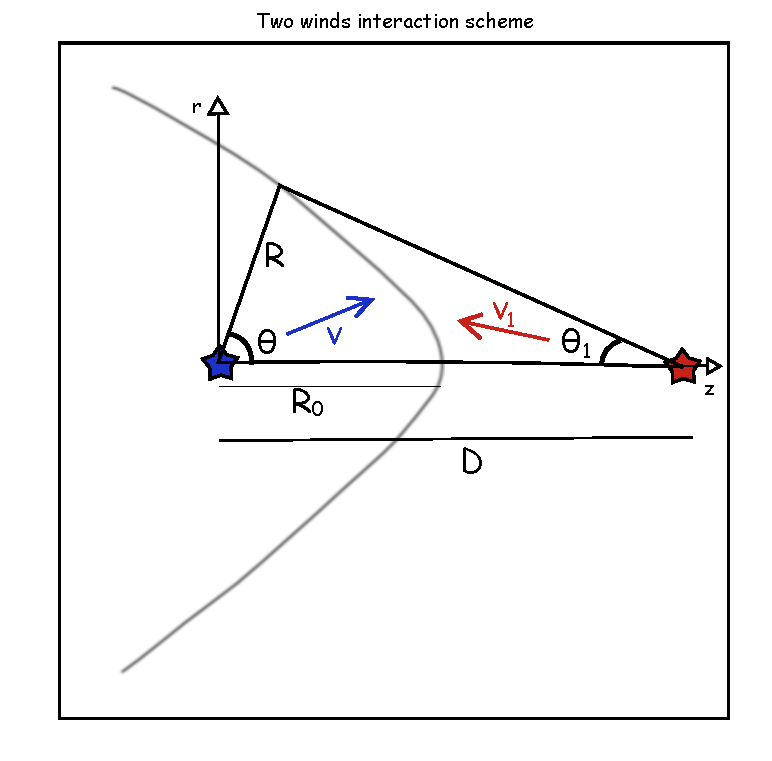
\includegraphics[width=\linewidth]{2winds-scheme}
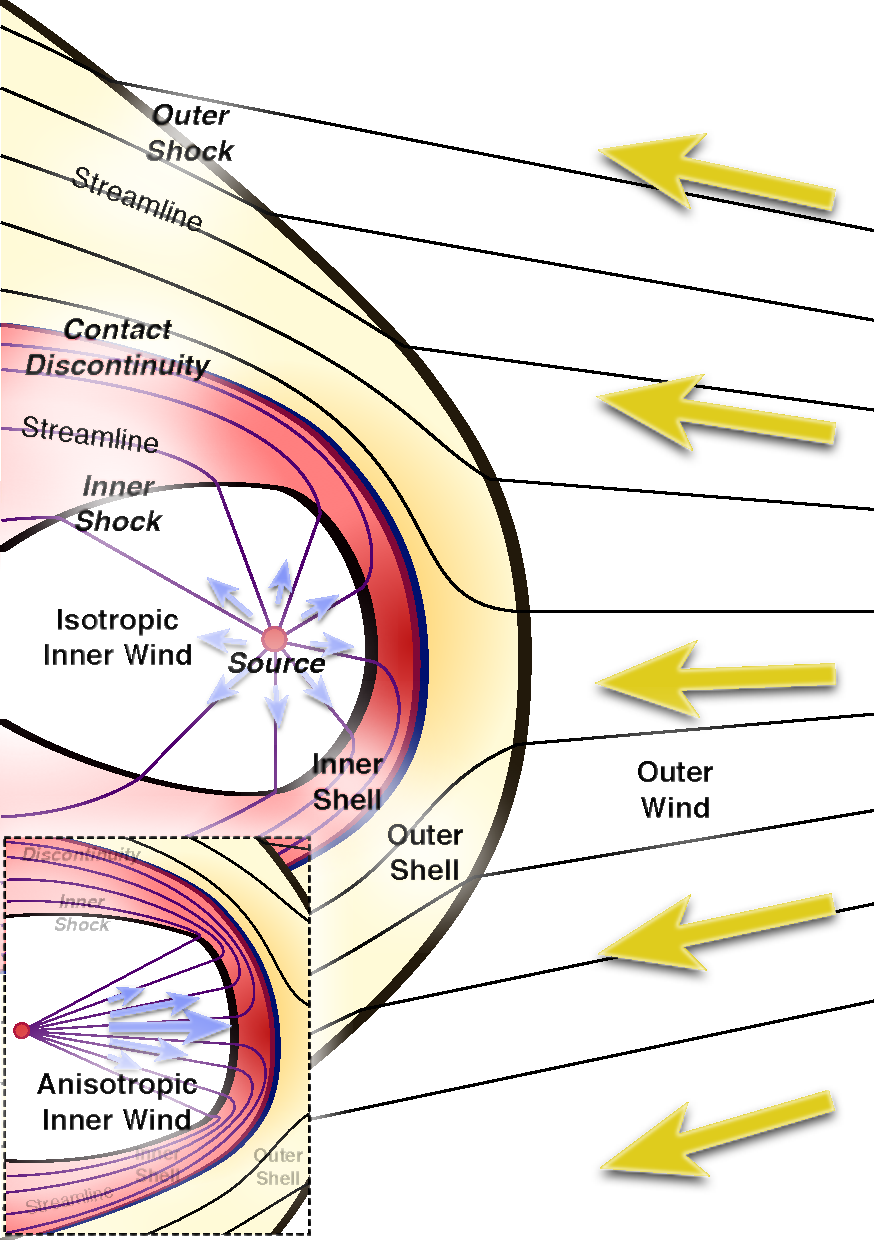
\includegraphics[width=\linewidth]{figs/generic-bowshock}
\caption{Quasi-stationary bow shock structure formed by the
  interaction of two supersonic winds.  Lower-left inset box shows the
  case where the inner wind is anisotropic.   
  % the two winds problem. Any point in the shell is located with the
  % coordinates $(R,\theta)$, and $\theta_1$ is measured from the
  % external wind position
}
\label{fig:2-winds}
\end{figure}

The general case of a two-wind interaction bow shock is illustrated in
Figure~\ref{fig:2-winds}.  If the winds are isotropic, then the bow
shock pattern wraps around the weaker of the two sources, in 

The bow shocks we consider are originated by a source located at the origin, emitting a wind with a mass loss rate of $\dot{M}_w$ and a terminal
(supersonic) velocity $v_w$. This wind interacts with another wind originated by another source located at a distance $D$ from the first one. 
The mass loss rate of the second source is $\dot{M}_{w1}$ and the terminal velocity is $v_{w1}$. The momentum of the wind of the second source is
higher than the momentum of the first one, and the resultant bow shock is stationary due to pressure balance. 

\subsection{Characteristic Radii}

In order to contrast different bow shock models, we  derive a set of measurable radii. Each model used should predict them and these predictions can be
compared with observations.

\begin{itemize}
\item Radius at axis of symmetry. Denoted as $R_0$. 
\item Radius of Curvature at the axis of symmetry. Denoted as $R_c$
\item Radius at the  perpendicular direction to the symmetry axis. Denoted as $R_{90}$
\item For open bow shocks, the asymptotic angle. Denoted as $\theta_\infty$
\end{itemize} 

\begin{figure}
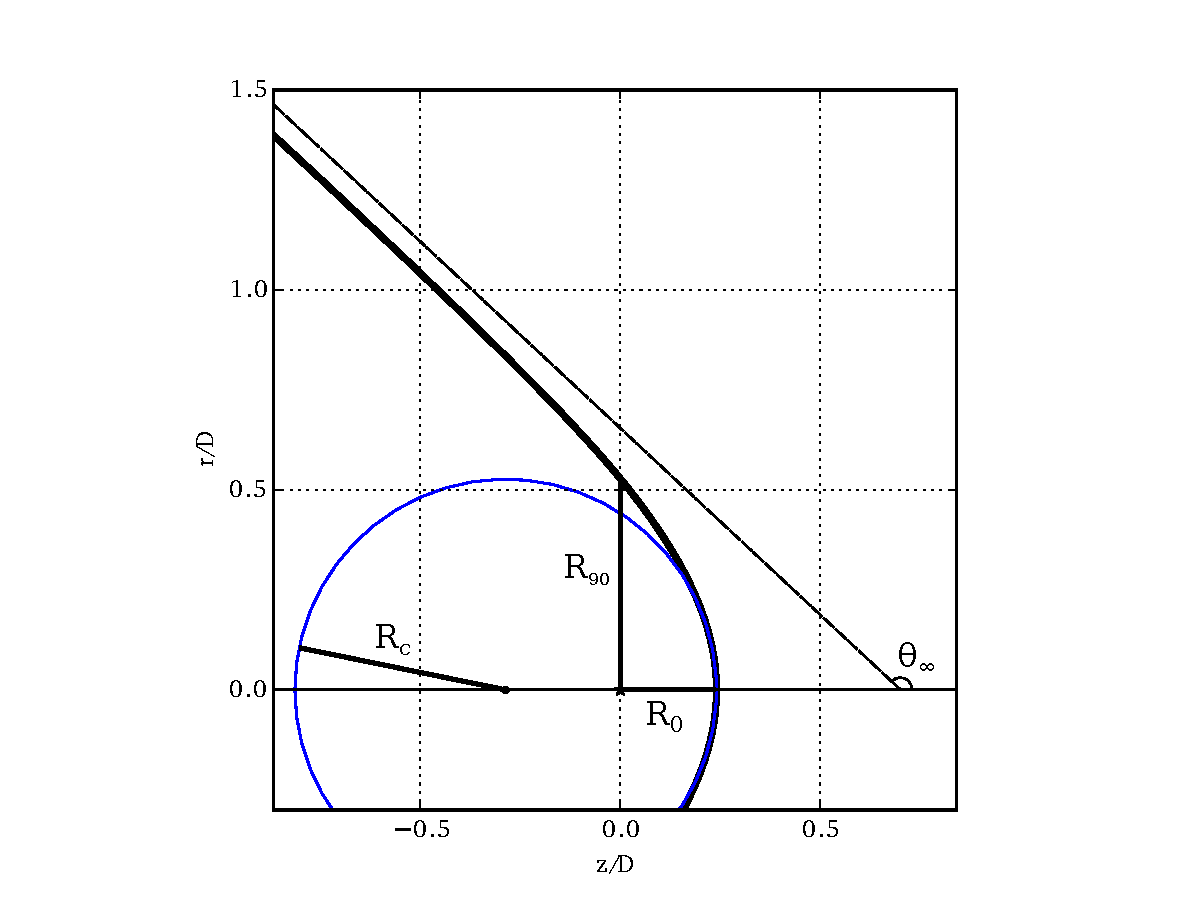
\includegraphics[width=\linewidth]{ch-radii_ed2}
\caption{Schematic representation of the characteristic radii $R_0$, $R_{90}$ and the radius of curvature at the symmetry axis $R_c$}
\end{figure}



%%% Local Variables:
%%% mode: latex
%%% TeX-master: "proplyd-bowshocks"
%%% End:

\newenvironment{Vector}{\left(\begin{array}{c}}{\end{array}\right)}
\newcommand\uvec[1]{\bm{\hat{#1}}}
\newcommand\T{_{\mathrm{\scriptscriptstyle T}}}

\section{Projection onto the plane of the sky}
\label{sec:projection}

In this section we calculate the apparent shape on the plane of the
sky of the limb brightened border of a shock or shell that is
idealized as an arbitrary cylindrically symmetric surface.

%Note: I'm aware that some of this material should be moved to an appendix, but I think it will be a future edition.
\subsection{Frames of reference}
\label{sec:ref-frames}

Consider body-frame cartesian coordinates $(x,y,z)$, where \(x\) is
the symmetry axis, and spherical polar coordinates
\((R, \theta, \phi)\), where \(\theta\) is the polar angle and
\(\phi\) the azimuthal angle.  Since the surface is cylindrically
symmetric, it is can be specified as $R = R(\theta)$, so that
cartesian coordinates on the surface are:
\begin{equation}
  \begin{Vector}
    x \\ y \\ z
  \end{Vector} 
  = R(\theta)
  \begin{Vector}
    \cos\theta \\
    \sin\theta\cos\phi \\
    \sin\theta\sin\phi
  \end{Vector}.
  \label{eq:body-frame}
\end{equation} 
Suppose that the viewing direction makes an angle \(i\) with the
\(z\)~axis, so that we can define observer-frame coordinates
\((x', y', z')\), which are found by rotating the body-frame
coordinates about the \(y\)~axis:
\begin{equation}
  \begin{Vector}
    x' \\ y' \\ z'
  \end{Vector}
  = 
  \begin{Vector}
    x\cos i - z\sin i\\
    y \\
    z\cos i + x\sin i
  \end{Vector}.
  \label{eq:Trans}
\end{equation} 
The relationship between the two frames is illustrated in
Figure~\ref{fig:projection-pos}.  All quantities in the observer's
frame are denoted by attaching a prime to the equivalent quantity in
the body frame.  The celestial coordinates on the ``plane of the sky''
are given by \((x', y')\) with \(x'\) being the projected symmetry
axis of the surface, while the line of sight lies along \(-z'\).  The
inclination angle \(i\) is defined so that \(i = 0^\circ\) when the
surface is viewed perpendicular to its axis (\textit{side on}) and
\(i = 90^\circ\) when it is viewed along its axis (\textit{end on}).

\begin{figure}
  \centering
  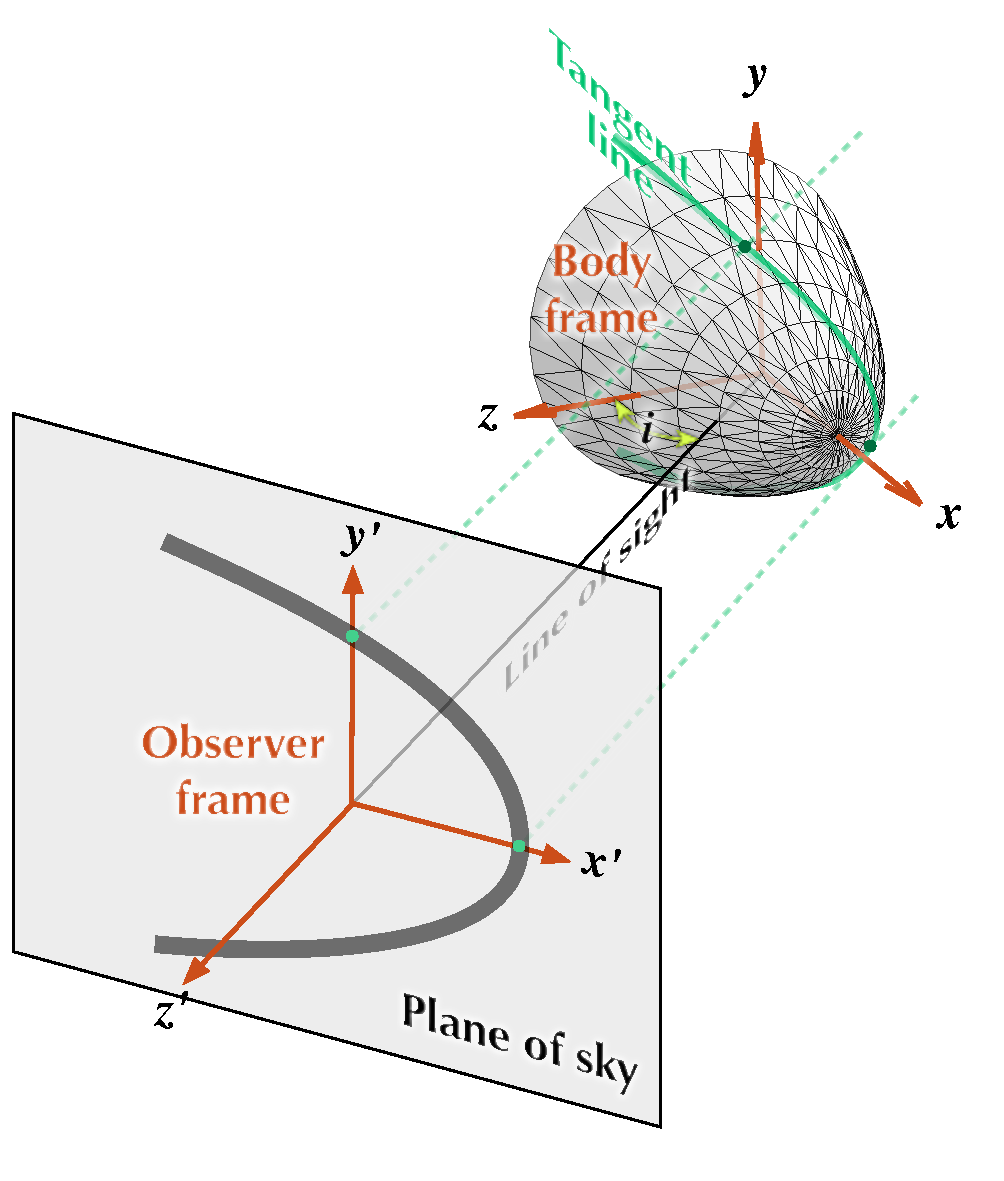
\includegraphics[width=\linewidth]{figs/projection-pos}
  \caption{Relationship between body frame (unprimed coordinates) and
    observer frame (primed coordinates).}
  \label{fig:projection-pos}
\end{figure}


%\subsection{Characteristic radii}
%\label{sec:characteristic-radii}
\begin{figure}
  \centering
  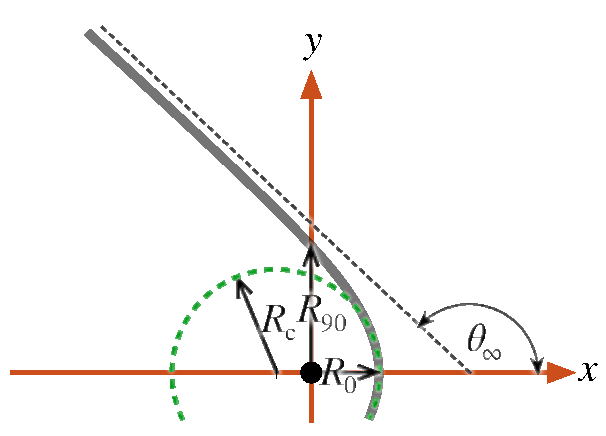
\includegraphics[width=\linewidth]{figs/characteristic-radii}
  \caption{Characteristic radii in the body frame.}
  \label{fig:characteristic-radii}
\end{figure}

\subsection{Unit vectors normal and tangential to the surface}
\label{sec:unit-vectors-normal}
\begin{figure}
  \centering
  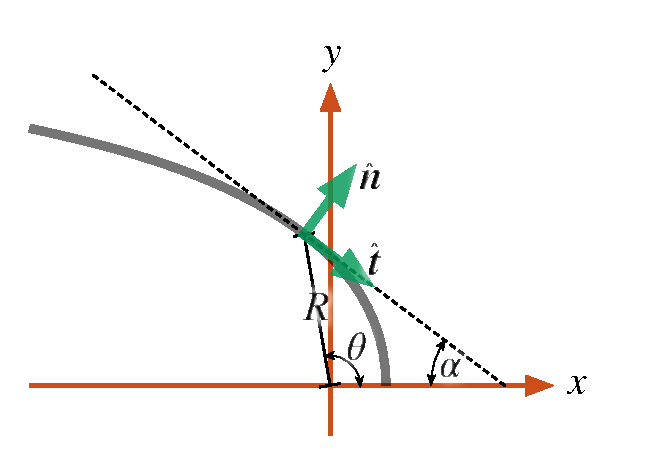
\includegraphics[width=\linewidth]{figs/bowshock-unit-vectors}
  \caption{Unit vectors in the body frame that are normal and
    tangential to the surface \(R(\theta)\) in a plane of constant
    azimuth, \(\phi\).}
  \label{fig:unitvec}
\end{figure}
We define unit vectors \(\uvec{n}, \uvec{t}\), such that \(\uvec{n}\) is normal to the surface, while \(\uvec{t}\) is tangent to the surface in a plane of constant \(\phi\). For \(\phi = 0\) the surface lies in the \(xy\) plane and it is straightforward to show (Fig.~\ref{fig:unitvec}) that in this case the unit vectors are given by 
\begin{equation}
  \label{eq:uvec-phi0}
  \uvec{t}_0 =
  \begin{Vector}
    -\cos\alpha \\ \sin\alpha \\ 0
  \end{Vector}
  \quad \mathrm{and} \quad
  \uvec{n}_0 =
  \begin{Vector}
    \sin\alpha \\ \cos\alpha \\ 0
  \end{Vector}, 
\end{equation}
where
\begin{equation}
  \label{eq:alpha}
  \tan\alpha = -\left.\frac{dy}{dx}\right\vert_{R(\theta)} 
  = \frac{1 + \omega \tan\theta}{\tan\theta - \omega}
\end{equation}
and 
\begin{equation}
  \label{eq:omega}
  \omega(\theta) = \frac{1}{R} \frac{dR}{d\theta} . 
\end{equation}
For general \(\phi\), \(\uvec{n}\) and \(\uvec{t}\) can be found by rotating equations~(\ref{eq:uvec-phi0}) around the \(x\)-axis, which can then be converted to the observer frame by use of equation~(\ref{eq:Trans}) to give
\begin{gather}
  \label{eq:nprime}
  \begin{split}
    \uvec{n}' = & \frac{1}{(1+\omega^2)^{1/2}} \\
    & \times 
      \begin{Vector}
        (\cos\theta+\omega\sin\theta)\cos i 
        - (\sin\theta-\omega\cos\theta) \sin i \sin\phi\\
        (\sin\theta-\omega\cos\theta)\cos\phi \\
        (\cos\theta+\omega\sin\theta)\sin i 
        + (\sin\theta-\omega\cos\theta)\sin\phi\cos i
      \end{Vector}\\
  \end{split}\\
  \label{eq:tprime}
  \begin{split}
    \uvec{t}' = & \frac{1}{(1+\omega^2)^{1/2}} \\
    & \times 
      \begin{Vector}
        -(\sin\theta-\omega\cos\theta)\cos i
        - (\cos\theta+\omega\sin\theta)\sin\phi\sin i \\
        (\cos\theta+\omega\sin\theta)\cos\phi \\
        -(\cos\theta+\omega\sin\theta)\sin i 
        + (\sin\theta-\omega\cos\theta)\sin\phi\cos i
      \end{Vector}
  \end{split}
  \end{gather}
\subsection{Tangent line}

% For optically thin emission with isotropic emissivity \(j\), the observed
% surface brightness for any line of sight that intersects the shell is
% \(S = \int j \, dz' / 4\pi\). 
 
% If the shell thickness is \(h(\theta)\) and emissivity is
% \(j(\theta)\), then for optically thin emission the observed
% surface brightness for any line of sight that intersects the shell is
% \(S = j s / 4\pi\), where \(s\)

% in the limit \(h \ll R\) and
% \(\mu\) is
% the cosine of the angle between the line of sight and the local normal
% to the shell surface at the point of intersection:
% \begin{equation}
%   \label{eq:2}
%   \mu = \uvec{n} \cdot \uvec{z}'
% \end{equation}

The boundary on the plane of the sky of the projected surface is the
locus of those lines of sight that graze the surface tangentially.
This corresponds to a curved line on the surface itself, which we
denote the \textit{tangent line}, and which is defined by the
condition  
\begin{equation}
  \label{eq:tangent-line-condition}
  \uvec{n}'\cdot \uvec{z}' = 0.
\end{equation}


We denote by \(\phi\T\) that value of $\phi$ that satisfies this
relation for a given inclination, \(i\), and polar angle, \(\theta\):
\begin{equation}
\sin\phi\T = \tan i\tan\alpha = \tan i \frac{1+\omega\tan\theta}{\omega-\tan\theta}
\label{eq:tanphi}
\end{equation}
From equations~(\ref{eq:body-frame}, \ref{eq:Trans}) it follows that
the observer-frame coordinates of the tangent line are given by
\begin{equation}
\left(\begin{array}{c}
x'\T \\ y'\T \\ z'\T
\end{array}\right)= R(\theta)\left(\begin{array}{c}
\cos\theta\cos i - \sin\theta\sin\phi\T \sin i \\
\sin\theta(1-\sin^2\phi\T)^{1/2} \\
\cos\theta\sin i +\sin\theta\sin\phi\T\cos i
\end{array}\right).
\label{eq:tangential}
\end{equation} 
Note that, in general, \(z'\T\) is not a linear function of \(x'\T\)
and \(y'\T\), so that the tangent line is not a plane curve. 

The apparent shape \((x'\T, y'\T)\) of the tangent line on the plane
of the sky can also be described in polar form as \(R'(\theta')\),
where
\begin{equation}
  \label{eq:R-prime-theta-prime}
  R' = (x'^2\T+ y'^2\T)^{1/2} 
  \quad \text{and} \quad
  \tan\theta' = y'\T / x'\T.
\end{equation}
It is important to note that equation~(\ref{eq:tanphi}) does not have
a solution for arbitrary values of $\theta$ and $i$, but only when
$|\tan i\tan\alpha|<1$. In particular, if $i\neq 0$, then the tangent
line only exists for \(\theta > \theta_{0}\) where \(\theta_{0}\) is
given implicitly by
\begin{align}
\tan\theta_{0} = \frac{|\tan i| + \omega(\theta_{0})}{1-\omega(\theta_{0}) |\tan i|} . 
\label{eq:thetapar}
\end{align}
In addition, if the surface is sufficiently ``open''
(\(\alpha > \alpha_{\mathrm{min}} > 0\) for all \(\theta\)), then for
those inclinations with
\(\vert i\vert > (90^\circ - \alpha_{\mathrm{min}}) \) the tangent
line does not exist for any value of \(\theta\).  In other words, when
the viewing angle is sufficiently close to face-on, the projected
surface has no ``edge'' and will no longer appear to be a bow shock.

\subsection{Characteristic radii on the plane of the sky}

Considering further applications to bow shocks, we will consider open shells. In order to compare the shell shape given by $R(\theta)$ with observations,
it is convenient to define the following apparent radii in the observer frame: $R'_{0}$ and $R'_{90}$. These are projected distances of the shell tangent line
from the origin. The first is measured in the direction of the symetry axis, and the second in a perpendicular direction. More concretely $R'_{0} = x'\T(y'\T=0)$
and $R'_{90} = y'\T(x'\T=0)$. From equations (\ref{eq:tanphi}) and (\ref{eq:tangential}) we find that:
\begin{align}
R'_{0} = R(\theta_{0})\cos(\theta + i) \label{eq:Rpar} 
\end{align}
Where $\theta_{0}$ is the solution of equation (\ref{eq:thetapar}), and
\begin{align}
R'_{90} = R(\theta_{90})\sin\theta_{90}\left(1-\sin^2(\phi\T(\theta_{90}))\right)^{1/2}
\end{align}
Where $\theta_{90}$ is the solution of the next implicit equation:
\begin{align}
\cot\theta_{90} = \frac{1-\left(1+\omega(\theta_{90})^2\sin^22i\right)^{1/2}}{2\omega(\theta_{90})\cos^2 i}
\end{align}


  \subsection{Line-of-sight velocities on the tangent line}
  \label{sec:line-sight-veloc}
  Motions in a thin shocked shell will be predominantly tangential to the shell surface. In addition, for the particular case of wind-wind bowshocks, the flow in each azimuthal slice can be shown to be independent \citep{Wilkin:2000a}, which implies that the shell velocity is parallel to \(\uvec{t}\). The projected line-of-sight shell velocity is therefore
  \begin{equation}
    \label{eq:vlos}
    v_{\mathrm{los}} = (\uvec{t}' \cdot -\uvec{z}') \, v_{\parallel}(\theta) = \frac{v_{\parallel}(\theta) (1+\omega^2)^{1/2} \sin i }{\sin\theta - \omega\cos\theta} ,
  \end{equation}
  where \( v_{\parallel}(\theta)\) is the gas velocity along the shell and the standard sign convention has been adopted such that velocities away from the observer are deemed positive. 


%%% Local Variables:
%%% mode: latex
%%% TeX-master: "proplyd-bowshocks"
%%% End:


\section{Conic section approximation to bow shock shapes}
\label{sec:conic}

\newcommand\Sin{\ensuremath{\mathcal{S}}}
\newcommand\Cos{\ensuremath{\mathcal{C}}}
\newcommand\Cot{\ensuremath{\mathcal{T}}}

In this section we will analyze the case where the resultant shape  of the bow shock is a conic curve (circle, ellipse, parabola or hyperbola).
These curves are mathematical simple to model and give us a good reference to understand the effects of the projection effects
described in the last section on other bow shocks. The source of the inner wind is located at the origin, and the center of the conic is located at
a distance $x_0$ from the source.

%Instead of the excentricity, we utilize the parameter $\theta_c$ to characterize the different curves, where
%$\tan\theta_c = \frac{b}{a}$,  $b$ and $a$ are the typical parameters of conics. A positive value for $\theta_c$ indicates that the given curve is a closed one, i.e
%an ellipse, while a negative value indicates that is an hyperbola. %Insert figures if neccesary  
\begin{figure}
\begin{tabular}{cc}
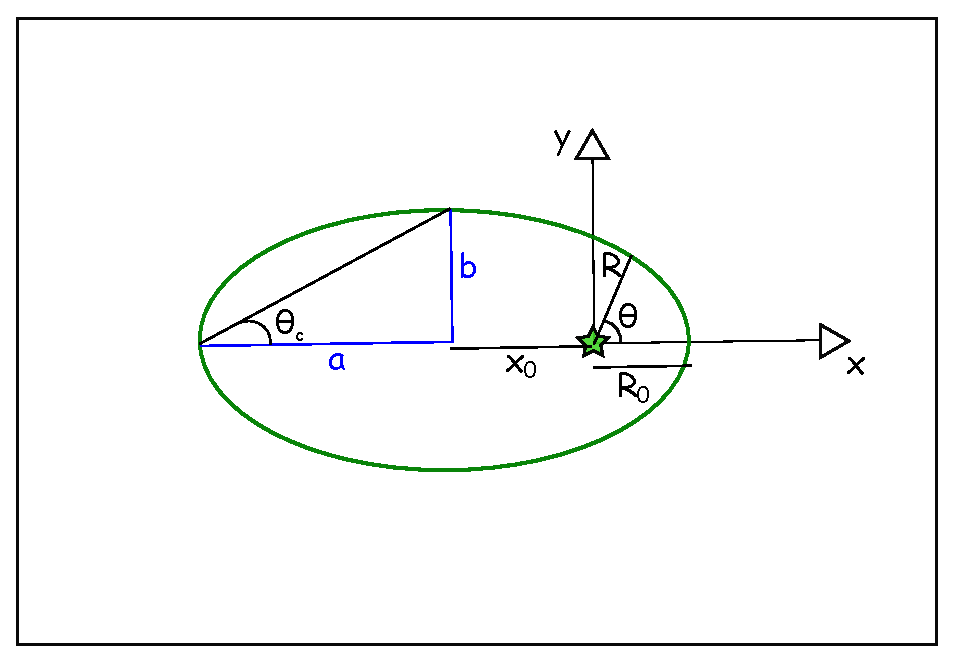
\includegraphics[width=0.4\linewidth]{ellipse} &
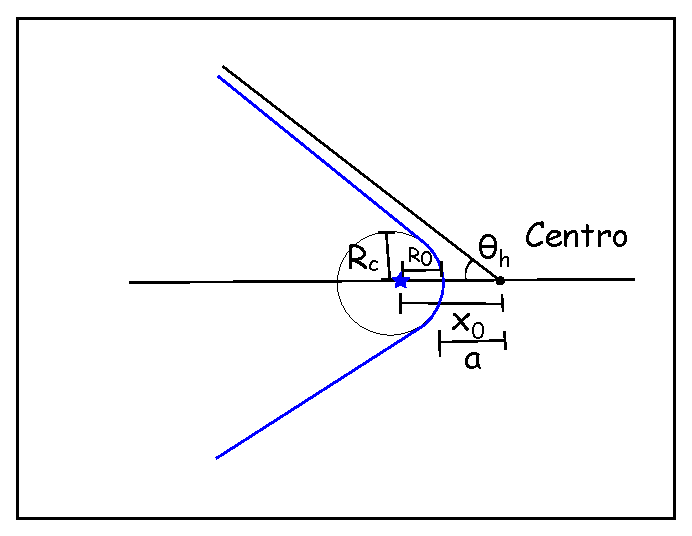
\includegraphics[width=0.4\linewidth]{hiperbola}
\end{tabular}
\label{fig:conics}
\caption{Schematic representation of conic like bowshocks: A) Ellipse and B) Hyperbola The center of the conic is located at a distance $x_0$ from the origin at the $x$ axis. The shell position is 
described either by cartesian coordinates $(x,y)$ or polar coordinates $(R,\theta)$. In this section is more convenient to use cartesian coordinates, as their parametrization is quite easy.}
\end{figure}
Due to the similitudes between the parametrization of the ellipse and the hyperbola, we can do the following parametrization:

\begin{align}
x = a\Cos(t)-x_0 \\ 
y = b\Sin(t)
\end{align}

where:
\begin{align}
\Cos(t) = \left\lbrace \begin{array}{c}
\cos t ~\mathrm{if~ellipse} \\
\cosh t ~\mathrm{if~hyperbola}
\end{array}\right.\\
\Sin(t) = \left\lbrace \begin{array}{c}
\sin t ~\mathrm{if~ellipse} \\
\sinh t ~\mathrm{if~hyperbola}
\end{array}\right. \\
-\pi < t < \pi \\
R_0 = a - x_0 \\
a<0 ~ \mathrm{for~hyperbola}
\end{align}
We have set a whole family of curves with a singular parameter denoted as $\tan\theta_c \equiv \frac{b}{a}$. Positive values of this parameter describe closed curves
(i.e. ellipses) and the negative ones describe open curves (i.e. hyperbolas). Particular cases are $\theta_c =\frac{\pi}{4}$, which describes a circle and $\theta_c=0$, which describes
a parabola.
\begin{figure}
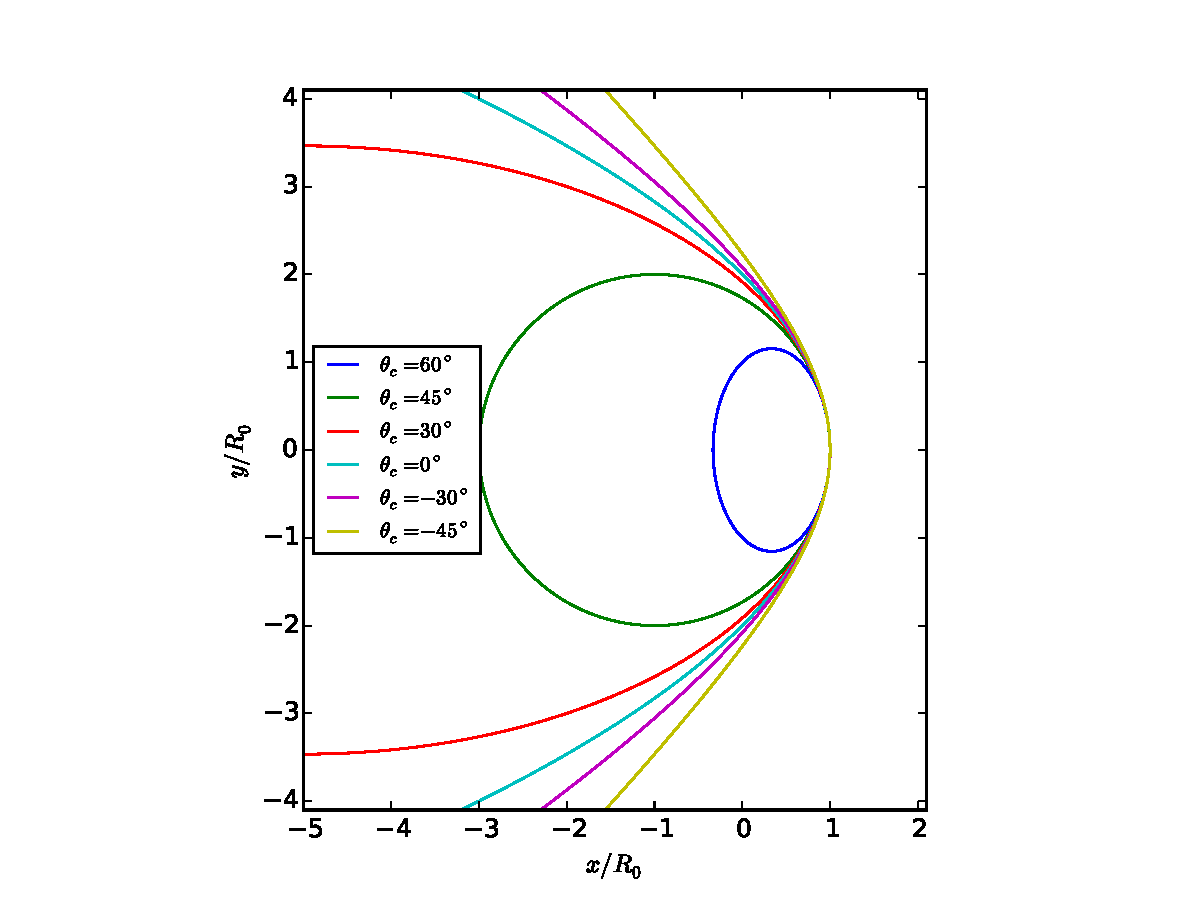
\includegraphics[width=\linewidth]{conic1}
\caption{A whole set of conics with the same radius of curvature. The parameter $\theta_c$ is used as the equivalent of the excentricity. This angle is defined as positive for closed curves
and negative forthe opened ones. An special case is $\theta_c=0$, which describes a parabola.}
\label{fig:conics-family}
\end{figure}
\subsection{Projection onto the plane of sky} 

Once the parametrization is done, we can find the apparent shape of the shell in the observer's frame, following the procedure explained in section \ref{sec:projection}.

First of all, the intrinsic 3D shape of the shell is given by:

\begin{align}
x = a\Cos(t)-x_0 \\ 
y = b\Sin(t)\cos\phi \\
z =  b\Sin(t)\sin\phi
\end{align}

The azimutal angle where the line of sight is tangent to the shell is given by equation (\ref{eq:tanphi}) and (\ref{eq:tanalpha}), then:

\begin{align}
\sin\phi_t &= \frac{b}{a}\tan i\Cot(t) 
\end{align}
where:

\begin{align}
\Cot(t) = \left\lbrace \begin{array}{c}
\cot t ~\mathrm{if~ellipse} \\
-\coth t ~\mathrm{if~hyperbola}
\end{array}\right.
\end{align}

We could work in another frame   where the origin is located at the conic's center: $(X,Y)$, where $X=x-X_0$ and $Y=y$.

In this frame,  we use the transformations (\ref{eq:Trans})  to obtain the apparent shape of the shell:

\begin{align}
X' = \frac{\Cos(t)}{a\cos i}\left(a^2\cos^2 i \pm b^2\sin^2 i\right)  \label{eq:conic-projected-x}\\
Y'= b\Sin(t)\left(1-\frac{b^2}{a^2}\tan^2 i\Cot(t)\right)^{1/2}
\label{eq:conic-projected-y}
\end{align}


We must show that the apparent shape of the shell in the observer's frame is still the same conic. To do that, we can write equations
(\ref{eq:conic-projected-x}) and (\ref{eq:conic-projected-y}) as follows:

\begin{align}
X' = a'\Cos t' \label{eq:conic-projected-x-2} \\
Y' = b'\Sin t' \label{eq:conic-projected-y-2}
\end{align}

Comparing, (\ref{eq:conic-projected-x}), (\ref{eq:conic-projected-x-2}), (\ref{eq:conic-projected-y}) and (\ref{eq:conic-projected-y}) we find that

\begin{align}
a' = \left(a^2\cos^2 i \pm b^2\sin^2 i\right)^{1/2} \\
\Cos(t') = \frac{\Cos(t)}{a\cos i} \\
b' = b
\end{align} 

Which proves that effectively the projection of a given conic is the same conic. With this knowledge, we can obtain the characteristic radii in
the observer's frame.

\begin{align}
D' = D\cos i \\
R'_0 = a' - (a-R_0)\cos i \\
R'_0 = \left(a^2\cos^2 i \pm b^2\sin^2 i\right)^{1/2}  - (a-R_0)\cos i
\end{align}

With  $f(i;\theta_c)\equiv\left(1\pm\tan^2\theta_c\tan^2i\right)^{1/2}$ and introducing the
radius of curvature $R_c\equiv \frac{b^2}{a}$ we find that:

\begin{align}
\frac{R'_0}{D'}=\frac{R_0}{D}\left(1+A\cot^2\theta_c(f(i;\theta_c)-1) \right)
\end{align}

Where $A\equiv \frac{R_c}{R_0}$

The Radius of curvature in the observer's frame is given by $R'_c=\frac{b'^2}{a'}$. Then:

\begin{align}
\frac{R'_c}{R'_0} = \frac{A}{\cos^2 i f(i;\theta_c)\frac{q'}{q}}
\end{align}

Where $q=\frac{R_0}{D}$ and $q' = \frac{R'_0}{D'}$
%Insert figures where needed

%%% Local Variables:
%%% mode: latex
%%% TeX-master: "proplyd-bowshocks"
%%% End:


\newcommand\thC{\(\theta^1\)\,Ori~C}
\defcitealias{Canto:1996}{CRW}
\newcommand\CRW{\citetalias{Canto:1996}}

\section{Application to the hypersonic thin shell solution}
\label{sec:crw-scenario}
As an example application of the ideas of this paper, we consider a
generalization of the thin-shell solution presented in
\citet[][hereafter \CRW{}]{Canto:1996}, for the interaction of two
hypersonic, constant velocity stellar winds.  It is assumed that the
two shocks are highly radiative and that the post-shock flows are
perfectly mixed to form a single shell of negligible thickness.  In
this approximation, the shape of the shell was found algebraically by
\CRW{} from considering conservation of linear and angular momentum,
following an approach first outlined in \citet{Wilkin:1996a}.  The
shape of the bow shock shell is uniquely determined by the parameter
\(\beta\), defined as the momentum-loss ratio of the two winds:
\begin{equation}
  \label{eq:beta-definition}
  \beta \equiv \frac{\dot{M}_w V_w}{\dot{M}_{w1} V_{w1}} . 
\end{equation}
In this definition we use the terminology of \CRW{}, in which
\(\dot{M}_w\) and \(V_w\) are the mass-loss rate and velocity,
respectively, of the wind with source at the origin, while
\(\dot{M}_{w1}\) and \(V_{w1}\) are the mass-loss rate and velocity of
the second wind, located at a distance \(D\) along their \(z\) axis.
Note that \CRW{}'s \(z\) and \(r\) correspond to \(x\) and \(y\) in
sections~\ref{sec:generic-model} to \ref{sec:conic} of the current
paper.  By always placing the weaker of the two winds at the origin,
it is only necessary to consider \(\beta \le 1\).
 
In this work the weakest wind is modeled as an anisotropic hemispherical radial wind
with the following density distribution:

\begin{align}
  n(\theta) = n_0\cos^k\theta
\end{align}  
The index $k$ gives the anisotropy degree. We are interested in winds where $k \geq 0$ for further applications. By the other side, we keep the strongest
wind as isotropic.

The shape of the resultant bow shock is given by:
%If we apply the \CRW{} formalism for a more generalized photoevaporated flow with density given by (\ref{eq:ngen}),
%we find that the solutions for equations (8) - (11) of \CRW{} are the following:

%If we apply the \CRW{} formalism for a generalized photoevaporated flow with density given by equation (\ref{eq:ngen}),
%the shell shape $R(\theta)$ may be calculated from equation (6) of CRW{}:
\begin{align}
  R = \frac{\dot{J}_w + \dot{J}_{w1}}{\left(\dot{\Pi}_{wr}+\dot{\Pi}_{wr1}\right)\cos\theta-\left(\dot{\Pi}_{wz1}+\dot{\Pi}_{wz1}\right)\sin\theta}
  \label{eq:Rmom}
\end{align}

Where:

\begin{align}
\dot{\Pi}_z &= \frac{v_w\dot{M}_w^0}{2(k+2)}\left(1-\cos^{k+2}\theta\right)  \label{eq:pir}\\
\dot{\Pi}_r &= \frac{1}{2}\dot{M}^0_w v_w I_k (\theta) \label{eq:piz}\\
I_k(\theta) & = \int^\theta_0 \cos^k \theta \sin^2\theta~d\theta \label{eq:Ik}\\
\dot{J}_w = 0 \label{eq:jdot} \\
\dot{M}_w &= \frac{\dot{M}_w^0}{2(k+1)}\left(1-\cos^{k+1}\theta\right) \label{eq:dotprop} \\
M^0_w &\equiv 4\pi v_w r^2_{IF} n_0 \bar{m}\\
\dot{\Pi}_{wz1} & = -\frac{\dot{M}^0_{w1}v_{w1}}{4}\sin^2\theta_1\\
\dot{\Pi}_{wr1} & = \frac{\dot{M}^0_{w1}v_{w1}}{4}\left(\theta_1-\sin\theta_1\cos\theta_1\right)\\
\dot{J}_{w1} & = \frac{\dot{M}^0_{w1}v_{w1}}{4}\left(\theta_1-\sin\theta_1\cos\theta_1\right)D \label{eq:jdot1}
\end{align}

Combining equations  (\ref{eq:pir}) to (\ref{eq:jdot1}) we can obtain numerically the bow shock shape $R(\theta)$ from equation (\ref{eq:Rmom}).
To find the projected shape in the plane of sky, we fit $R(\theta)$ into a quadric curve which has the same characteristic radii $(R_0,R_c,R_{90})$. 
%The most notable scenarios, since they have astrophysical relevance are the following:
%$k=1/2$ ak.a. the ``proplyd case'', following \citep{HA:1998}, and $k=0$, ak.a, the ``isotropic case'', following \CRW{}. The comparison between both solutions
%is shown in figure (\ref{fig:r-beta}), along with an extreme anisotropy case. 

\begin{figure}
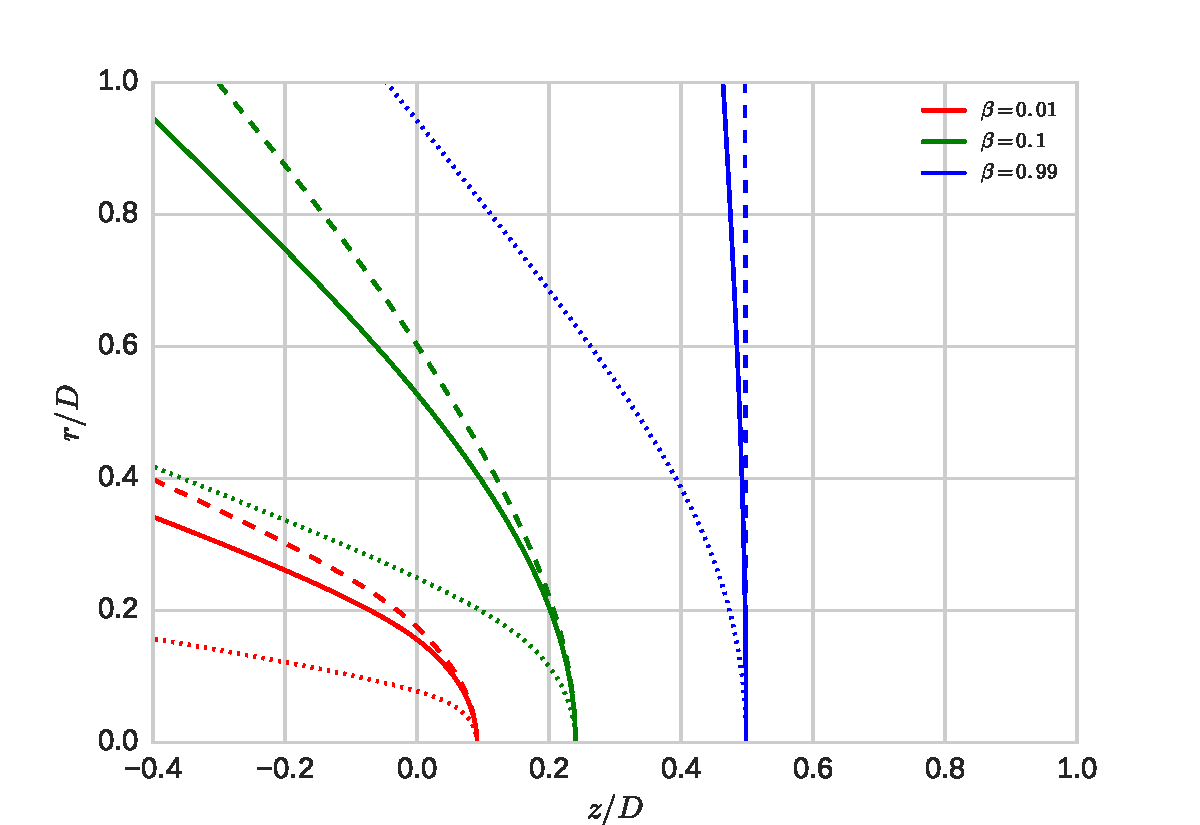
\includegraphics[width=\linewidth]{r-beta}
\caption{Bow shock shapes for interacting winds in the thin-shell
  approximation. Coordinates are normalized by $D$, the distance
  between the two wind sources.  The weaker source is at \((0.0, 0.0)\)
  and the stronger source is at \((1.0, 0.0)\).  Results are shown for
  different values of the wind momentum ratio, \(\beta\), and for the
  case where the weaker wind is isotropic (dashed lines) or an
  anisotropic photoevaporation flow. The solid lines shows a wind with a
  moderate degree of anisotropy $(k=0.5)$, which is expected for the proplyds.
  And the dooted lines show a wind with extreme anisotropy degree $(k=8)$.}
\label{fig:r-beta}
\end{figure}


\subsection{Characteristic Radii}
$R_0$ is obtained directly from equation (27) of \CRW{} as the distance from the inner source where the RAM pressure of the interacting winds is in equilibrium.
%Here goes a little introduction
For the rest of the radii we need a relation between $\theta$ and $\theta_1$ as follows:


\begin{align}
\theta_1\cot\theta_1 -1 = 2\beta I_k(\theta) \cot\theta - \frac{2\beta}{k+2}\left(1-\cos^{k+2}\theta\right)
\label{eq:th1th}
\end{align}

Equation (\ref{eq:th1th}) is reduced to equation (24) of \CRW{} when $k=0$.
We can obtain $R_{90}$ by following the process shown in appendix \ref{app:r90-analytic},
which lead us to a solution for $B \equiv \frac{R_{90}}{R_0}$:

\begin{align}
B = \frac{\sqrt(3\xi)\left(1+\beta^{1/2}\right)}{(1-\xi\beta)\left(1+\frac{1}{5}\xi\beta\right)^{1/2}}
\label{eq:B}
\end{align}

Now, the solution for $R_c$ is explained in appendix \ref{app:rc-analytic},
which lead us to derive the radius of curvature at the symmetry axis:

\begin{align}
R_c &= R_0\left(1-2\gamma\right)^{-1} \label{eq:Rcurv} \\
\mathrm{where:~} & \gamma = \frac{C_{k\beta}}{1+\beta^{1/2}}+\frac{1}{6}(1-2\beta^{1/2})
\end{align}

Finally, using equations (\ref{eq:Rcurv}) and (\ref{eq:B}) we can estimate the parameter of
conic curves $\theta_c$ as a function of $(\beta,\xi)$ using equation (\ref{eq:thc-conic})

\begin{align}
\tan^2\theta_c &= \left| \frac{3\xi\left(1+\beta^{1/2}\right)^2}{\left(1-\xi\beta\right)^2\left(1+\frac{1}{5}\xi\beta\right)}-\frac{2}{\left(1-2\gamma\right)}\right| 
\label{eq:thc-CRW}
\end{align}

\begin{figure}
\begin{tabular}{c}
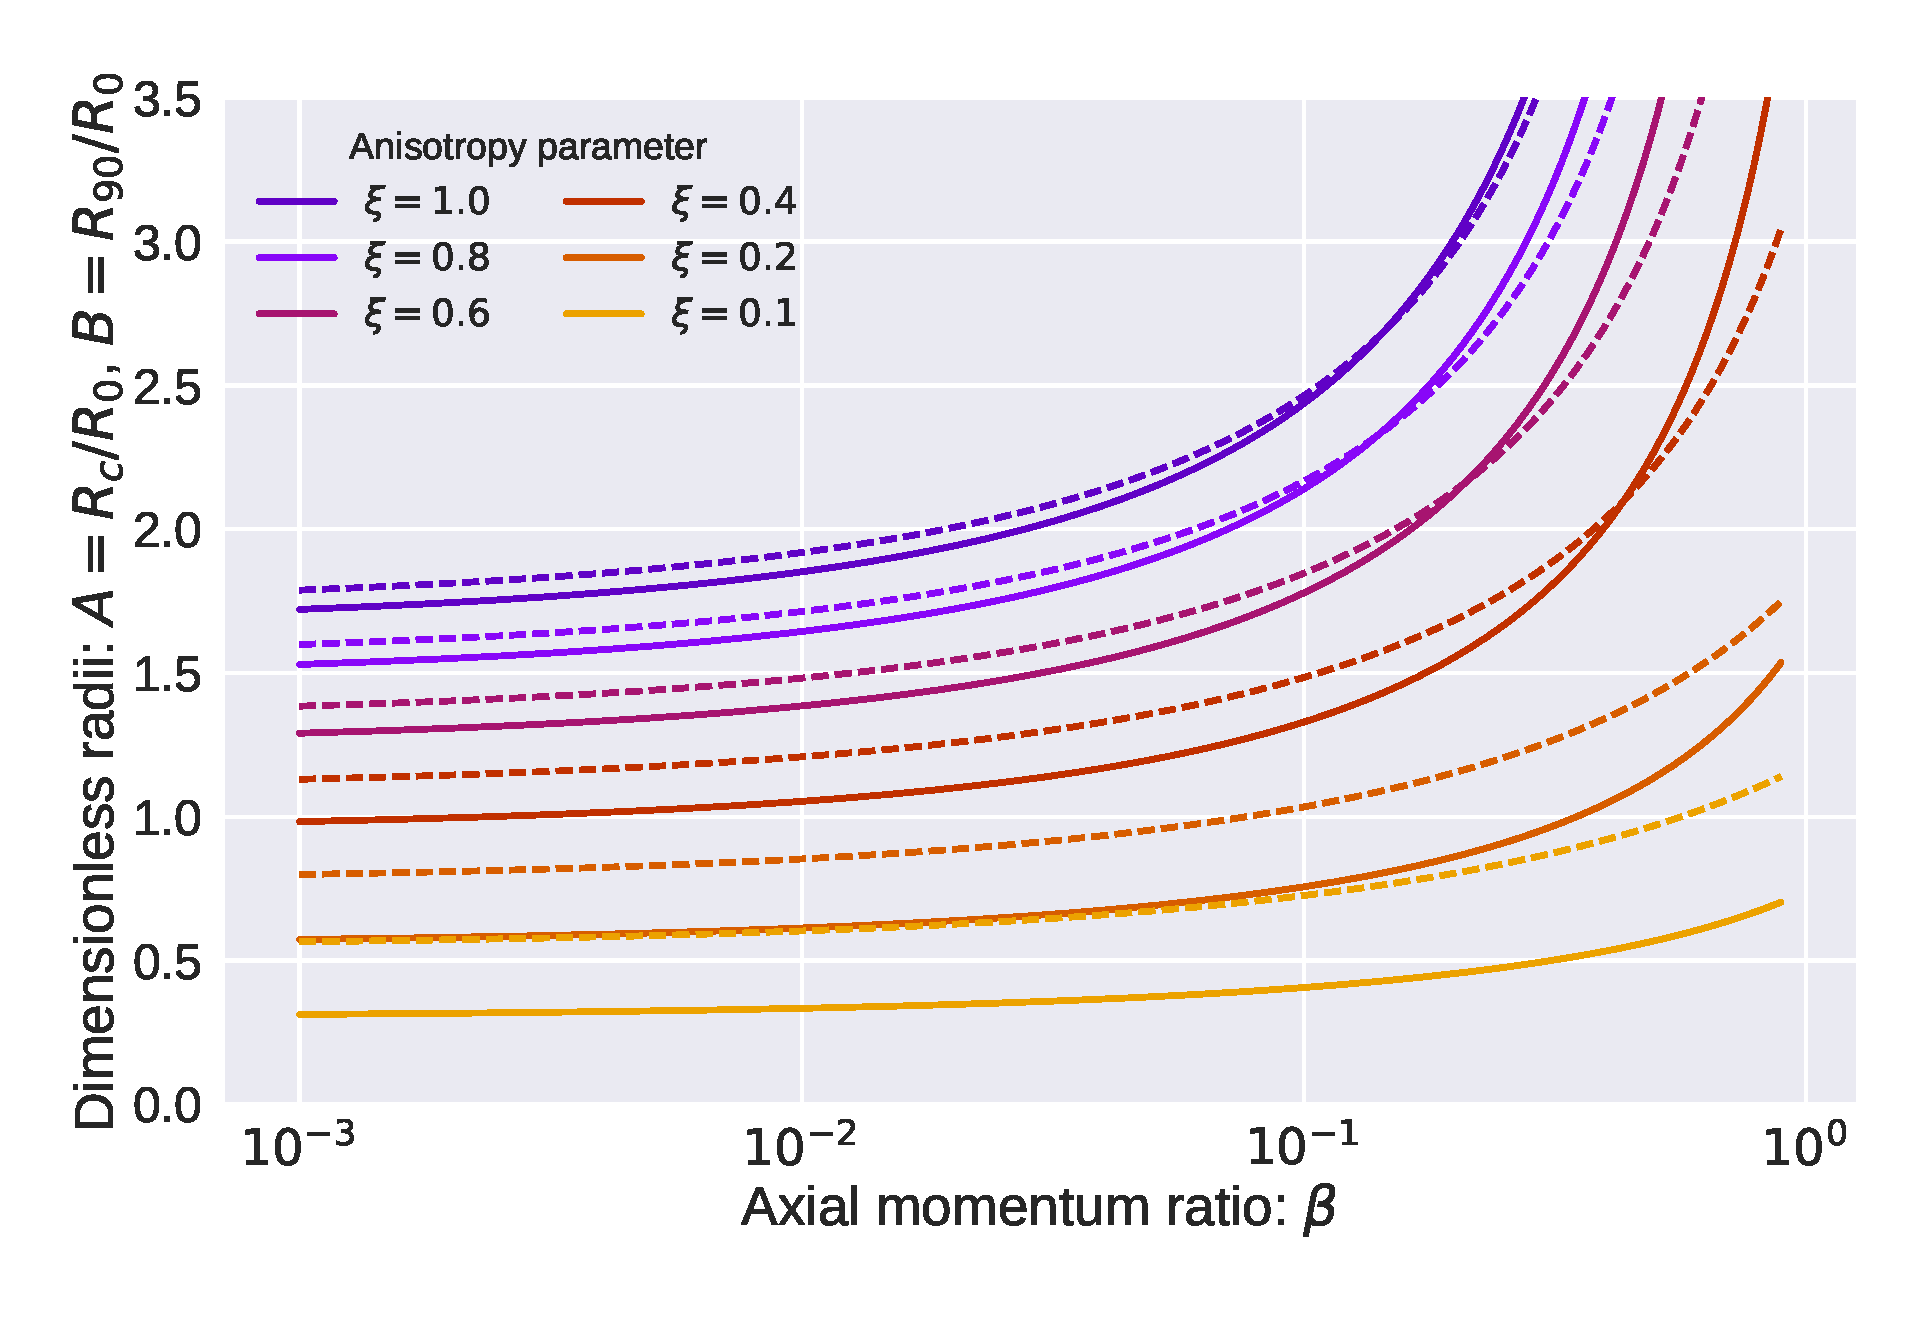
\includegraphics[width=\linewidth]{figs/AB-beta-log} \\
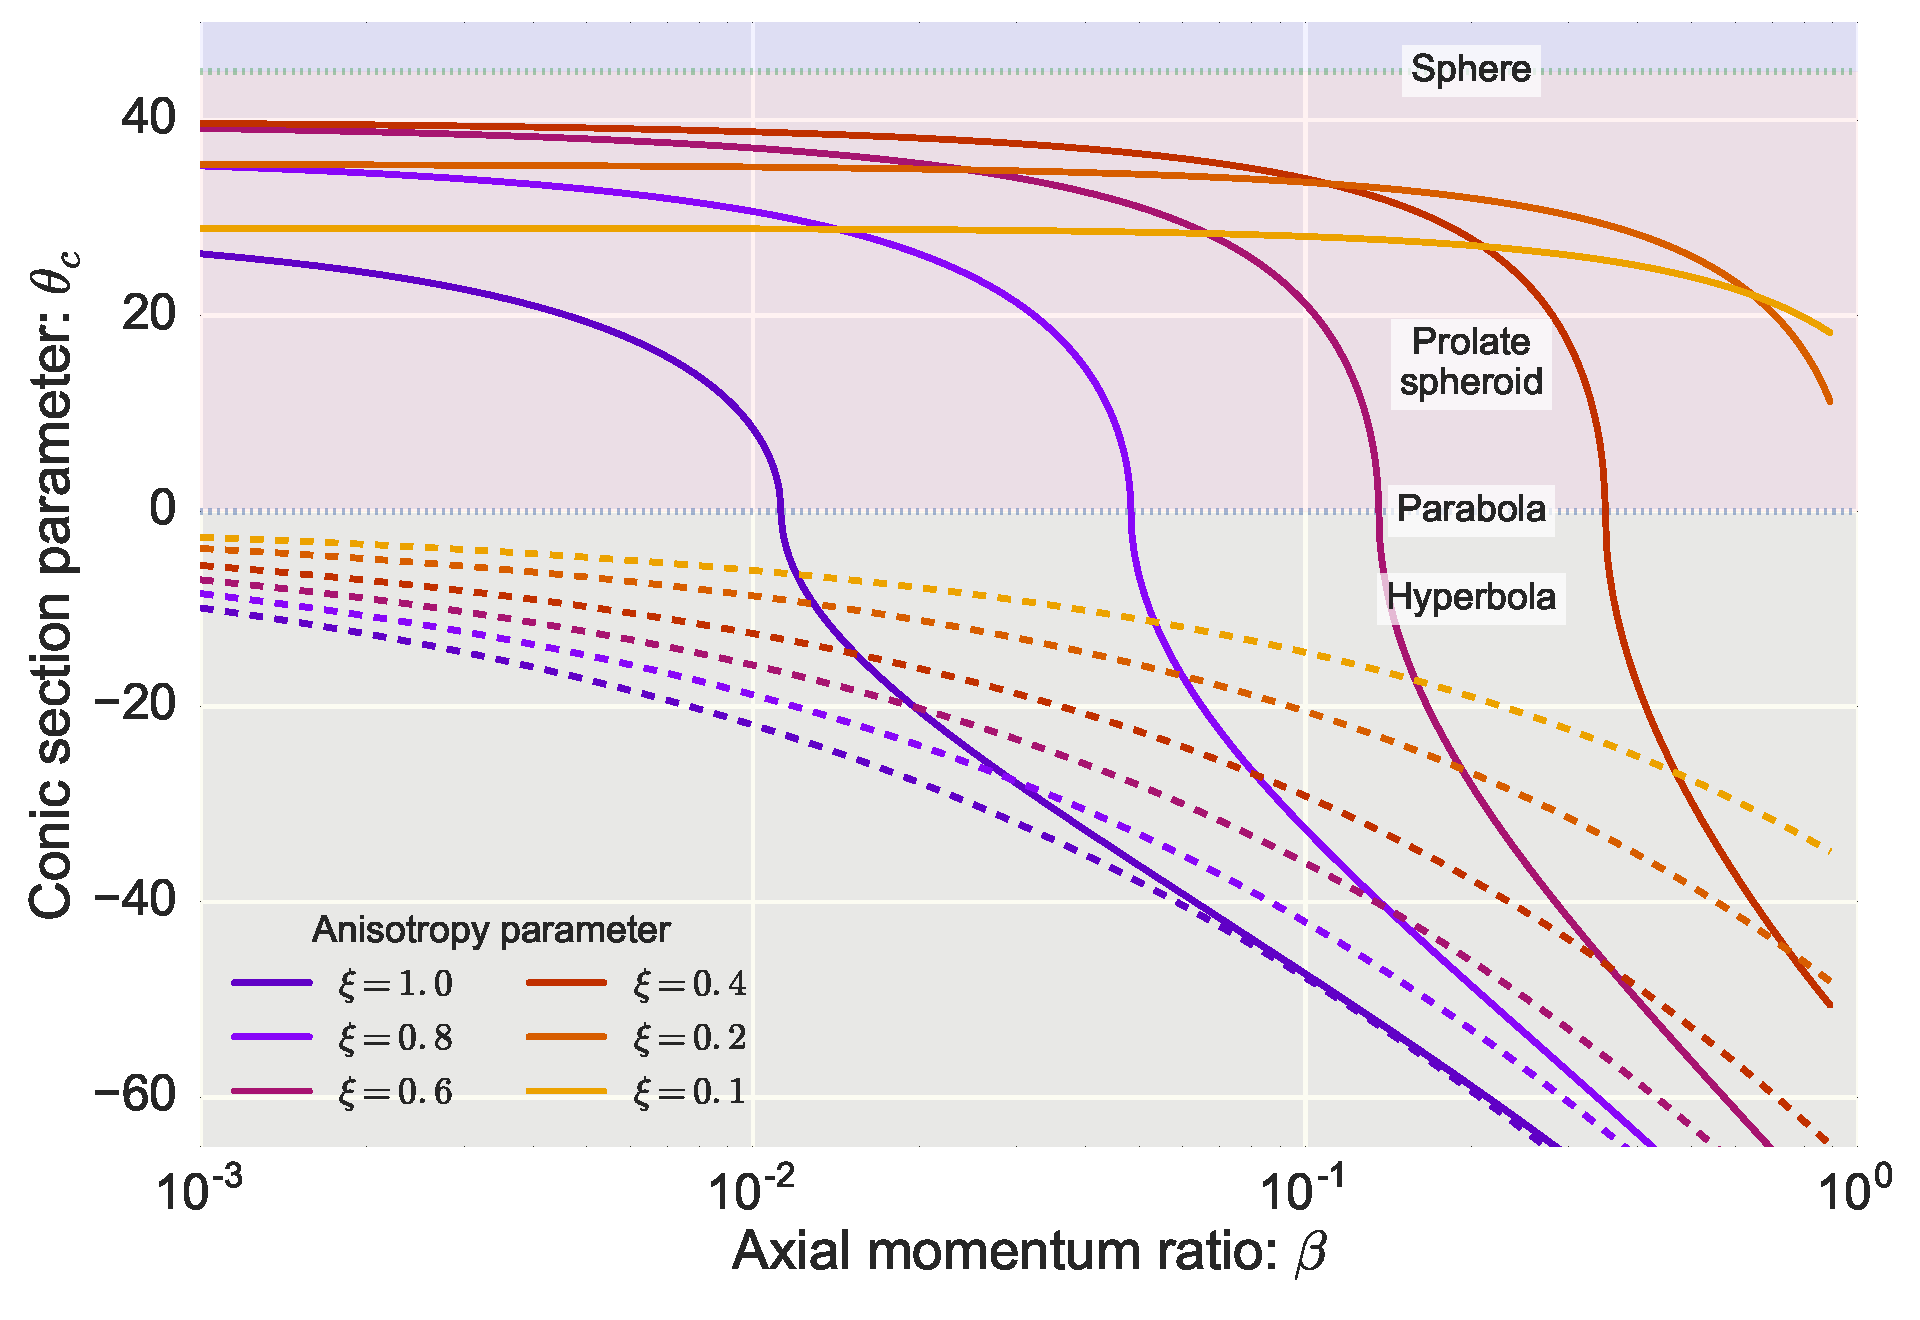
\includegraphics[width=\linewidth]{figs/thc-beta-log}
\end{tabular}
\caption{Top: Characteristic radii, $A = R_c/R_0$ (solid lines) and $B
  = R_{90}/R_0$ (dashed lines)
  vs $\beta$, calculated from quadric fits to the generalized CRW
  solutions with varying degrees of isotropy $\xi$.  Bottom: Conic
  angle $\theta_c$ vs $\beta$ for the bow 
  shock head (solid lines) and the bow shock tail (dashed lines).}
\label{fig:rad-beta}
\end{figure}


%Observationally, we can measure the projected radii. In order to estimate the model parameters is neccesary to measure at least two of the mentioned radii, being $R_0$ the
%easiest to measure. Therefore, we may compare both $R_c$ and $R_{90}$ against $R_0$ as shown in figure (\ref{fig:prop-shell-rad}). 

With this we can use the results of section \ref{sec:conic} to estimate the projected conic shapes for bow shocks with different winds 
momenta and different density distributions. Figure \ref{fig:rad-beta} shows equations ( \ref{eq:B}), (\ref{eq:Rcurv}) and (\ref{eq:thc-CRW}) for different anisotropy indexes. 


\subsection{Fits to the tail}
\label{sec:fits-tail}


For the hyperbola ``center''
\begin{multline}
  \label{eq:tail-analytic-x0}
  x_{0,\mathrm{t}} = 0.7 \beta^{-0.55} \biggl[
    C_3 \bigl(\log_{10}\beta\bigr)^3 + C_2 \bigl(\log_{10}\beta\bigr)^2 
  \\ + C_1 \log_{10}\beta + C_0
  \biggr]
\end{multline}
\begin{equation}
  \label{eq:tail-analytic-x0-minus-a}
  (x_{0,\mathrm{t}} - a_{\mathrm{t}}) = D_2 (\log_{10}\beta)^2 + D_1 \log_{10}\beta + D_0
\end{equation}
where
\begin{alignat}{2}
  C_k &= c_{2,k} \xi^2 + c_{1,k} \xi + c_{0,k} &\quad \text{for\ } k &= \{0, 1, 2, 3\} \\
  D_k &= d_{2,k} \xi^2 + d_{1,k} \xi + d_{0,k} &\quad \text{for\ } k &= \{0, 1, 2\} \\
  \label{eq:tail-analytic-coeffs}
\end{alignat}


\newcommand\iso{\ensuremath{^{\mathrm{iso}}}}

\begin{table}
  \caption{Coefficients for hyperbola fit to bowshock tails}
  \label{tab:tail-fit-coeffs}
  \begin{align*}
  C\iso_0 & = {0.123}  & c_{0,0} & = {0.123} & c_{1,0} & = {0.123} & c_{2,0} & = {0.123} \\
  C\iso_1 & = {0.123}  & c_{0,1} & = {0.123} & c_{1,1} & = {0.123} & c_{2,1} & = {0.123} \\
  C\iso_2 & = {0.123}  & c_{0,2} & = {0.123} & c_{1,2} & = {0.123} & c_{2,2} & = {0.123} \\
  C\iso_3 & = {0.123}  & c_{0,3} & = {0.123} & c_{1,3} & = {0.123} & c_{2,3} & = {0.123} \\
  D\iso_0 & = {0.123}  & d_{0,0} & = {0.123} & d_{1,0} & = {0.123} & d_{2,0} & = {0.123} \\
  D\iso_1 & = {0.123}  & d_{0,1} & = {0.123} & d_{1,1} & = {0.123} & d_{2,1} & = {0.123} \\
  D\iso_2 & = {0.123}  & d_{0,2} & = {0.123} & d_{1,2} & = {0.123} & d_{2,2} & = {0.123} \\
  \end{align*}
\end{table}




\begin{figure*}
  \centering
  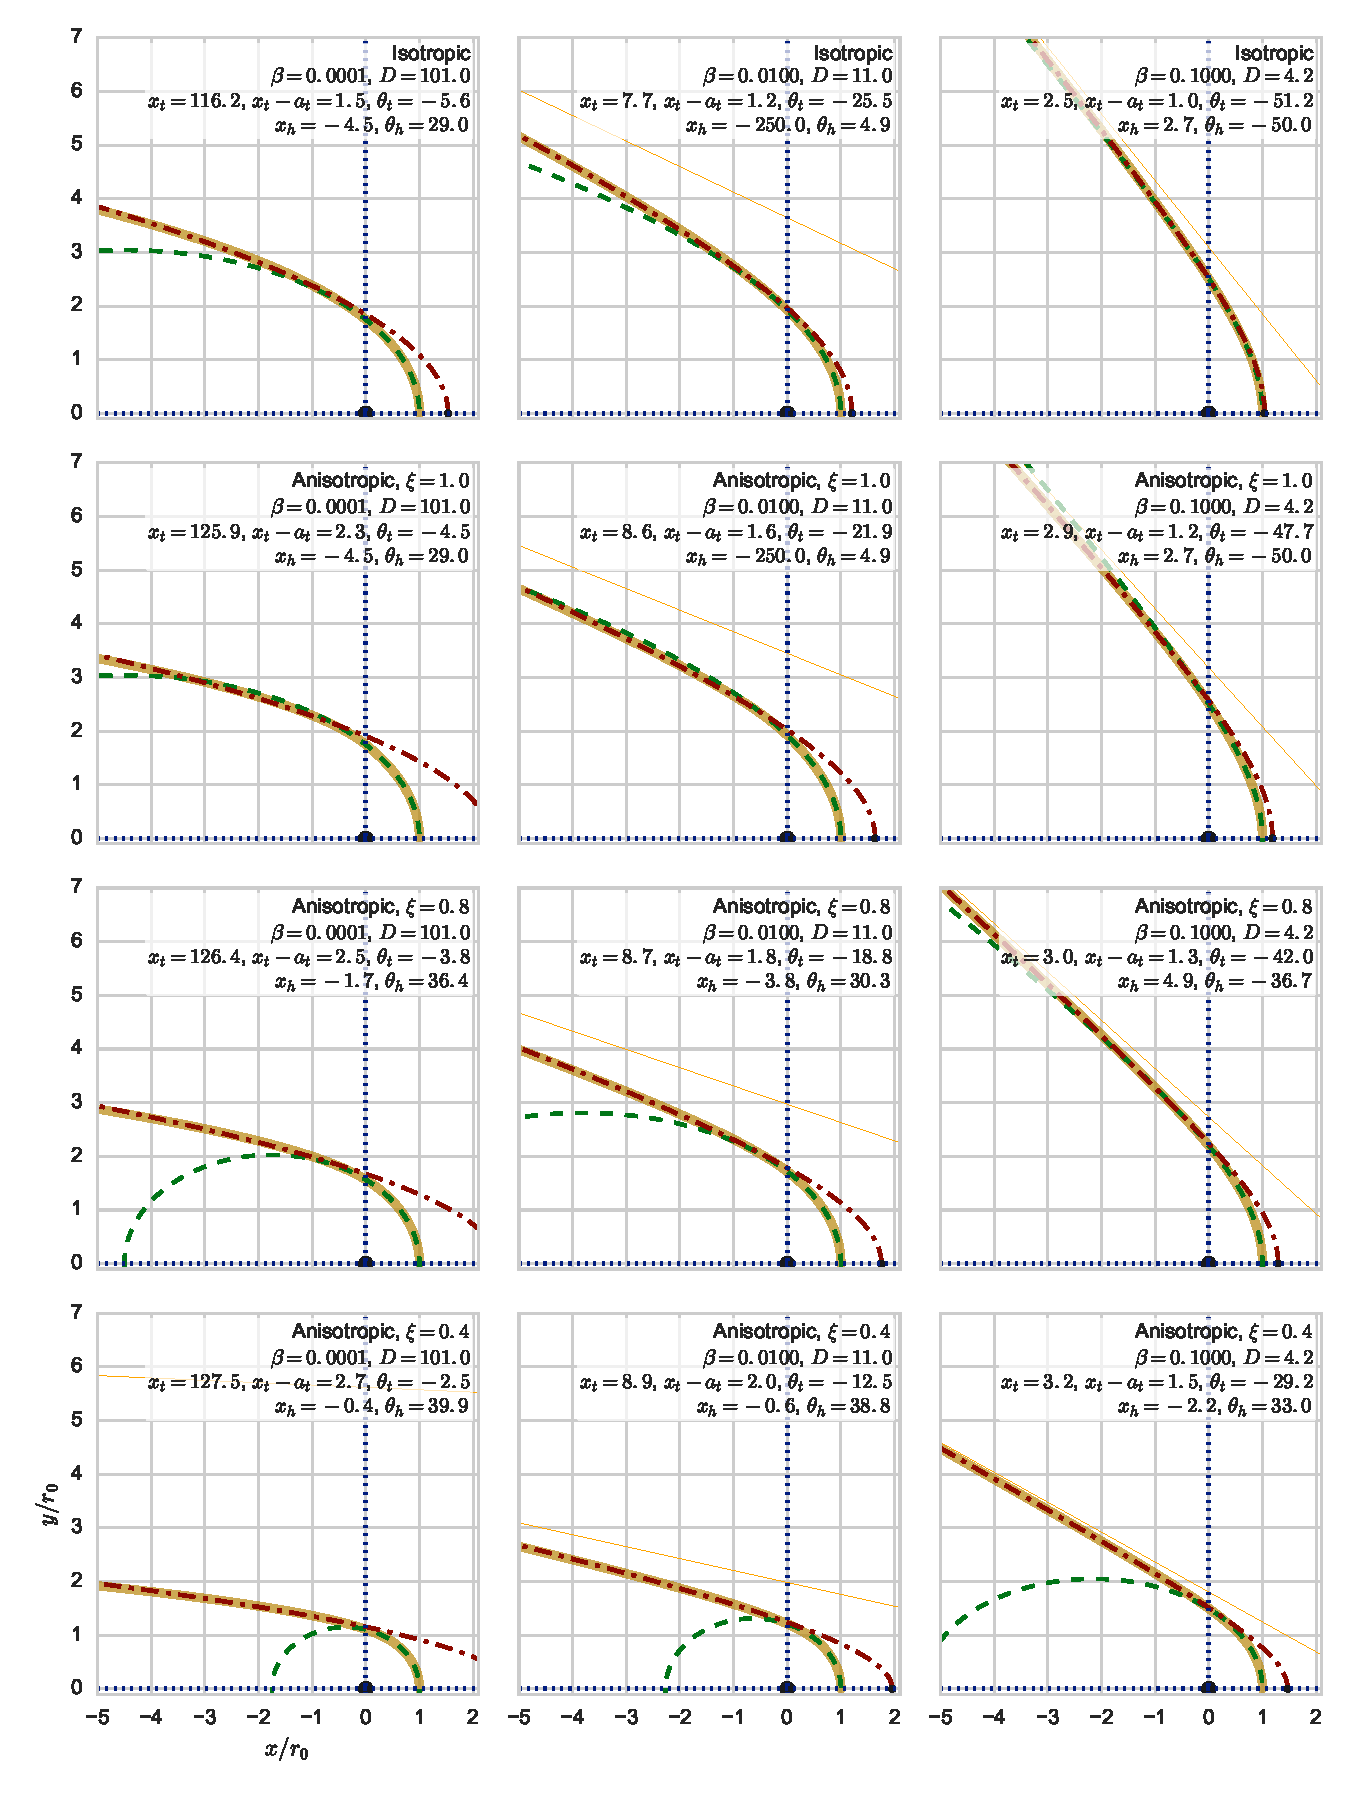
\includegraphics[width=\linewidth]{figs/conic-head-tail-fit}
  \caption{Double quadric fits to thin shell
    solutions. \textit{Replace these with a version that uses analytic
    fit to tail hyperbola parameters}}
  \label{fig:head-tail}
\end{figure*}

%%% Local Variables:
%%% mode: latex
%%% TeX-master: "quadrics-bowshock"
%%% End:

% 
\section{Shape of a dusty radiative bow wave}
\label{sec:shape-dust-wave}

As an alternative to hydrodynamic or magnetohydrodynamic bow shocks,
it is possible that some observed emission arcs may be bow waves due
to the action of radiation pressure on dust grains.

\begin{figure}
  (a)\\
  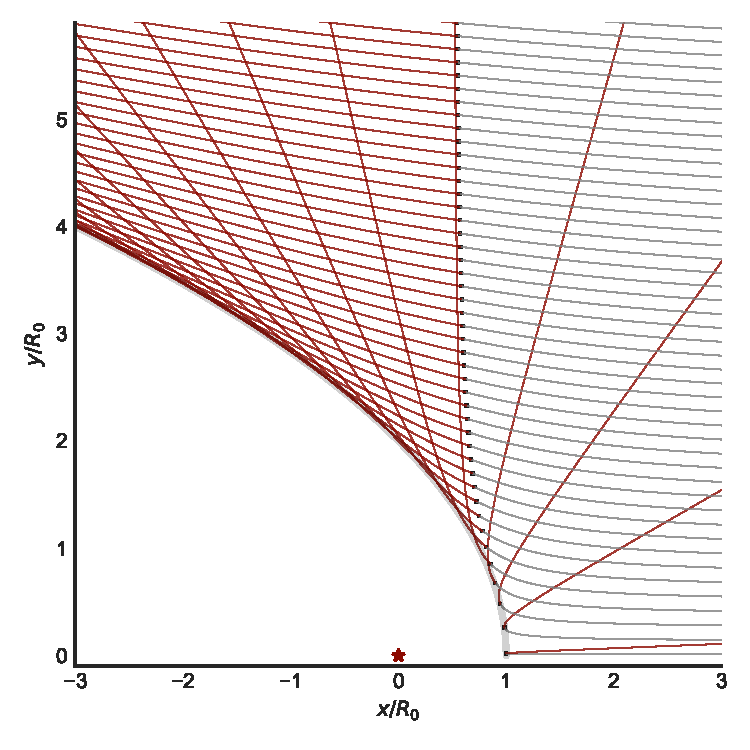
\includegraphics[width=\linewidth]{figs/dust-trajectories}
  (b)\\
  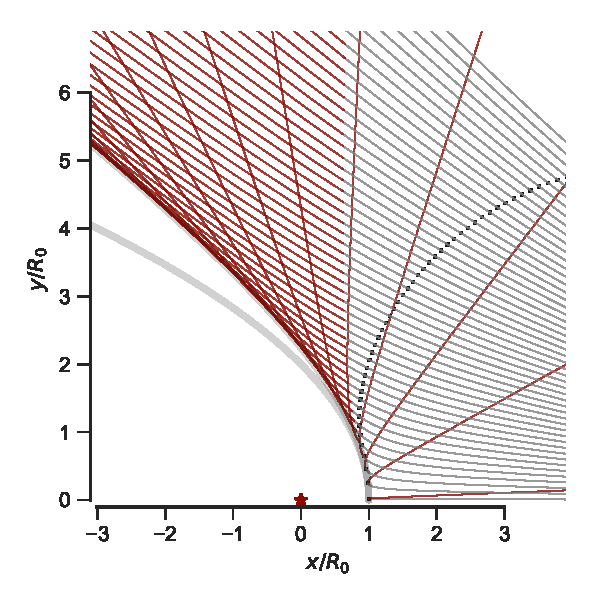
\includegraphics[width=\linewidth]{figs/dust-divergent}
  \caption[Dust grain trajectories]{Dust grain trajectories under
    influence of a repulsive central \(r^{-2}\) radiative force.
    (a)~A parallel stream of dust grains approach from the right at a
    uniform velocity and with a variety of impact parameters (initial
    \(y\)-coordinate). The central source is marked by a red star at
    the origin, and its radiative force deflects the trajectories into
    a hyperbolic shape, each of which reaches a minimum radius marked
    by a small black square.  The incoming hyperbolic trajectories are
    traced in gray and the outgoing trajectories are traced in red.
    The locus of closest approach of the outgoing trajectories is
    parabolic in shape (traced by the thick, light gray line) and this
    constitutes the inner edge of the bow wave.  (b)~The same but for
    a divergent stream of dust grains that originates from a source on
    the \(x\) axis at a distance \(D = 10 R_0\) from the origin.  In
    this case, the inner edge of the bow wave is hyperbolic and the
    parallel stream result is also shown for comparison.}
  \label{fig:dust-trajectories}
\end{figure}



A dust grain of geometrical cross-section \(\xsec\) situated a
distance \(R\) from a point source of radiation with luminosity \(L\)
will experience a repulsive, radially directed radiative force
\citep[e.g.,][]{Spitzer:1978a}
\begin{equation}
  \label{eq:dust-rad-force}
  \frad = \frac{\xsec \Qp L} {4 \pi R^2 c} e^{-\tau}
\end{equation}
where \Qp{} is the frequency-averaged\footnote{%
  Frequency averages of any quantity \(x\) should be understood as
  weighted by the attenuated source spectrum:
  \(\langle x \rangle_\nu = (L \, e^{-\tau})^{-1} \int_0^\infty x(\nu)\, L_\nu \, e^{-\tau_\nu} \, d\nu
  \).  } %
radiation pressure efficiency\footnote{%
  For absorption efficiency \(Q_{\text{abs}}\), scattering efficiency
  \(Q_{\text{scat}}\), and asymmetry parameter (mean scattering
  cosine) \(g\), we have
  \(\Qp = Q_{\text{abs}} + (1 - g) Q_{\text{scat}}\)
  \citep[e.g., \S~4.5 of][]{Bohren:1983a}.} %
of the grain, \(c\) is the speed of light, and \(\tau\) is the
frequency-averaged optical depth between the source and the grain.
For simplicity, we will consider only the optically thin case,
\(\tau \to 0\).

\subsection{Gas-free bow wave}
\label{sec:gas-free-bow}


If \(\frad\) is the only force experienced by the grain, then it will
move on a \textit{ballistic} trajectory, determined by its initial
speed at large distance, \(v_\infty\), and its impact parameter, \(b\).
For \(b = 0\), the grain radially approaches the source with initial
radial velocity \(-v_\infty\), which is decelerated to zero at the distance
of closest approach, \(R_0\), given by energy conservation:
\begin{equation}
  \label{eq:dust-r0}
  R_0 = \frac{\xsec \Qp L} {2 \pi c m\grain v_\infty^2} \ ,
\end{equation}
where \(m\grain\) is the grain mass.  The grain then turns round and
recedes from the source along the same radius, reaching a velocity of
\(+v_\infty\) at large distance.  For \(b > 0\), the trajectory,
\(R\grain(\theta; b)\), is found\footnote{%
  The problem is formally identical to that of Rutherford scattering,
  or (modulo a change of sign) planetary orbits.  The method of
  solution (via introduction of a centrifugal potential term and
  reduction to a 1-dimensional problem) can be found in any classical
  mechanics text \citep[e.g.,][\S~14]{Landau:1976a}.} %
to be hyperbolic, characterized by an eccentricity,
\(\varepsilon = \bigl( 1 + 4 b^2 / R_0^2\bigr)^{1/2}\), and polar angle of
closest approach, \(\thm = \cos^{-1} \varepsilon^{-1}\).  The trajectory is
symmetrical about \(\thm\) and can be written as
\begin{equation}
  \label{eq:dust-r-theta}
  \frac{R\grain(\theta; b)} {R_0} = 
  \frac{ \tfrac12 \bigl( \varepsilon^2 - 1 \bigr)} {\varepsilon \cos(\theta - \thm) - 1} \ , 
\end{equation}
with a total deflection angle of \(2 \thm\), which is equal to
\ang{90} when \(b = 0.5 R_0\).

\subsubsection{Parallel dust stream}
\label{sec:dust-parallel}

If the incoming dust grains initially travel along parallel
trajectories with varying \(b\), but the same \(v_\infty\), then deflection
by the radiative force will form a bow wave around the radiation
source, as shown in Figure~\ref{fig:dust-trajectories}.  However, the
inner edge of the bow wave, \(R_{\text{in}}(\theta)\) is not given by the
closest approach along individual trajectories, \(R\grain(\thm; b)\),
but instead must found by minimizing \(R\grain(\theta; b)\) over all
\(b\) for each value of \(\theta\), which yields
\begin{equation}
  \label{eq:dust-r-in}
  \frac{R_{\text{in}}(\theta)} {R_0} = \frac{2}{1 + \cos\theta} \ .
\end{equation}
This is the polar form of the equation for the confocal parabola,
which we have already discussed in detail in \PaperI{}'s
\S~\ref{Q-sec:conic} and Appendix~\ref{Q-app:parabola}.  Its planitude
and alatude are \(\Gamma = \Lambda = 2\) and these are unchanged under projection
at any inclination.



\subsubsection{Divergent dust stream}
\label{sec:dust-divergent}

If the dust grains are assumed to originate from a second point
source, located at a distance \(D\) from the radiation source, then
the incoming stream will be divergent instead of plane parallel.  The
individual streamlines are not affected by this change and are still
described by equation~\eqref{eq:dust-r-theta}, except that the
trajectory axes for \(b > 0\) are no longer aligned with the global
symmetry axis, so we must make the substitution
\(\theta \to \theta + \theta_1(b)\), where \(\sin \theta_1 = b / D\) (see
Fig.~\ref{Q-fig:crw-schema} of \PaperI{}). We parametrize the degree
of divergence as \(\mu = R_0 / D\) and, as before,
\(R\grain(\theta + \theta_1(b, \mu); b)\) is minimized over all trajectories to
find the shape of the bow wave's inner edge.  This time, the result is
a confocal hyperbola:
\begin{equation}
  \label{eq:dust-divergent-r-in}
  \frac{R_{\text{in}}(\theta; \mu)} {R_0} = \frac{1 + \varepsilon_\mu}{1 + \varepsilon_\mu\cos\theta} \ ,
\end{equation}
where the eccentricity is (to first order in \(\mu\))
\( \varepsilon_\mu = (1 - 2\mu)^{-1}\).  An example is shown in
Figure~\ref{fig:dust-trajectories} for \(\mu = 0.1\).  Unsurprisingly,
the resulting bow shape is more open than in the parallel stream case,
increasingly so with increasing \(\mu\).  The planitude and alatude are
both equal: \(\Pi = \Lambda = 1 + \varepsilon_\mu\).

\newcommand\drag{\ensuremath{_{\text{drag}}}}
\newcommand{\gas}{\ensuremath{_{\text{gas}}}}
\newcommand{\drift}{\ensuremath{_{\text{drift}}}}
\newcommand\soundspeed{\ensuremath{c_{\text{s,gas}}}}


\begin{figure}
  \centering
  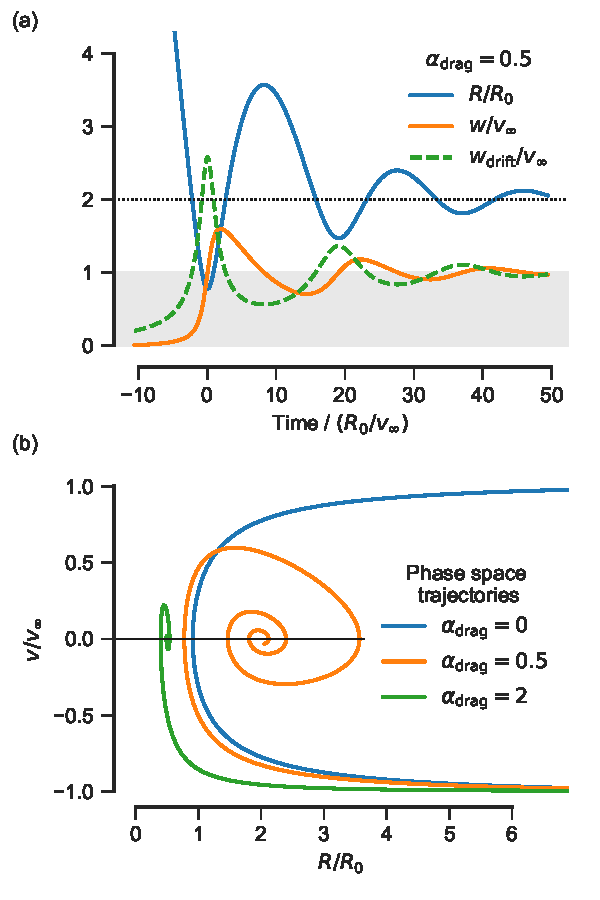
\includegraphics[width=\linewidth]{figs/dust-coupling-1d}
  \caption{Dust-gas coupling for an on-axis (purely radial)
    trajectory.  (a)~Grain radial position, \(R/R_0\), gas--grain
    velocity difference, \(w/v_\infty\), and local asymptotic drift
    velocity, \(w\drift/v_\infty\), versus time for
    \(\alpha\drag = 0.5\).  The behavior is typical of the dynamics of a
    damped harmonic oscillator. (b)~Phase space (position, velocity)
    trajectories for \(\alpha\drag = 0\), 0.5, and 2. All trajectories
    begin in the lower right corner and evolve in a clockwise
    direction. For \(\alpha\drag > 0\), the grain spirals in on the point
    \((x, u) = (\alpha\drag^{-1}, 0)\).}
  \label{fig:dust-coupling-1d}
\end{figure}

\begin{figure*}
  \centering
  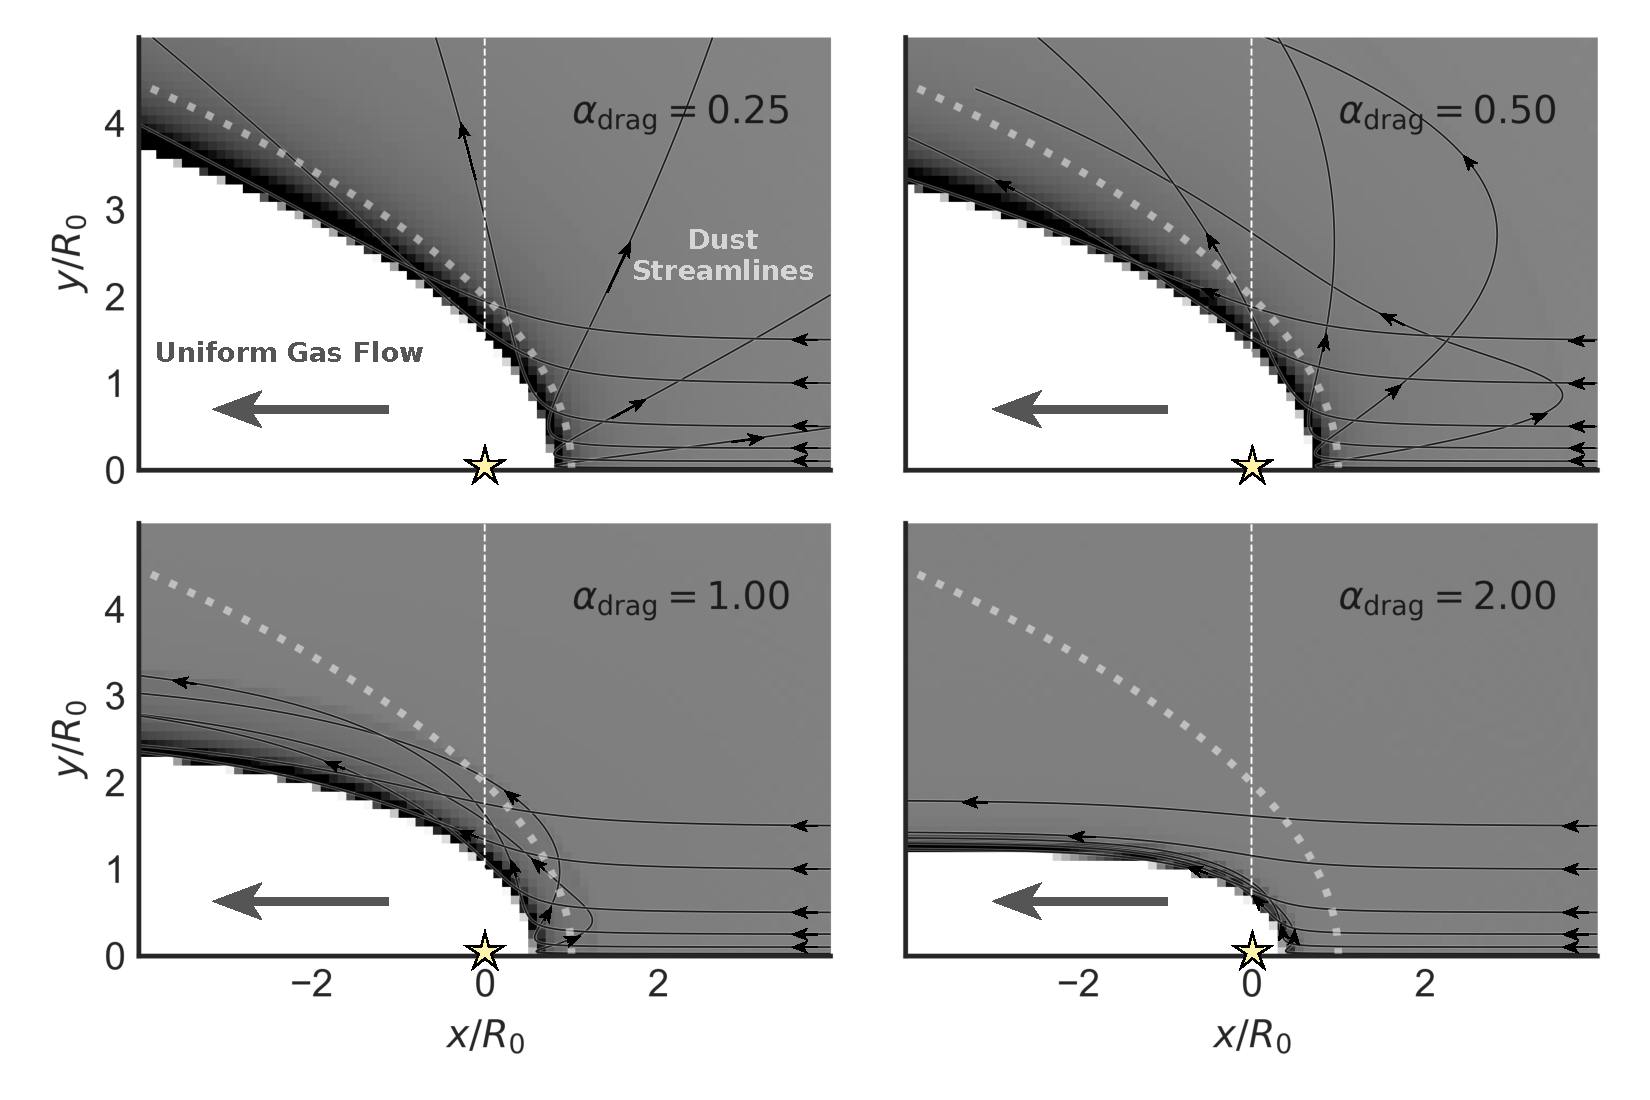
\includegraphics[width=\linewidth]{figs/dust-couple-stream-annotate}
  \caption{Dust grain trajectories under influence of gas drag in
    addition to a repulsive central radiative force.  The dust
    streamlines are shown as black lines with arrows and the dust
    density as a linear gray scale, with maximum (black) of twice the
    ambient dust density.  Results are shown for four values of the
    drag parameter (see text): \(\alpha_\text{drag} = 0.25\), \(0.5\),
    \(1.0\), and \(2.0\). The shape of the bow wave for the drag-free
    case (Fig.~\ref{fig:dust-trajectories}) is shown by the thick
    dotted line.  Faint patterns visible in the density away from the
    bow wave are numerical aliasing artefacts caused by sparse
    sampling of the streamlines in the low density regions.}
  \label{fig:dust-wave-coupling}
\end{figure*}


\subsection{Bow wave with gas drag}
\label{sec:bow-wave-drag}
More realistically, a grain will also be subject to a drag force,
\(f\drag\), due to its relative motion with respect to gas or plasma
particles. If the gas density, velocity, and sound speed are
\(\rho\gas\), \(v\gas\), and \(\soundspeed\), then a grain with velocity
\(v\grain\) will experience a drag force that is directed opposite to
the relative velocity, \(\bm{w} = \bm{v}\grain - \bm{v}\gas\).  In the
supersonic limit, \(w \equiv \abs{\bm{w}} \gg \soundspeed\), the magnitude of
the force is
\begin{equation}
  \label{eq:dust-fdrag}
  \abs{f\drag} \approx Q\drag \xsec \rho\gas w^2 \ ,
\end{equation}
where \(Q\drag\) is an efficiency factor (which may be smaller or
greater than unity) that accounts for details such as sticking
probability and the boost in cross section due to the Coulomb force
when a charged grain interacts with an ionized plasma
\citep{Draine:1979a}.  We neglect the back reaction of the dust on the
gas motion and assume a uniform background gas flow that is perfectly
coupled to the incoming dust stream at large radii.  So, for the
parallel stream case, we have \(\bm{v}\gas = -v_\infty \uvec{x}\) everywhere.

Considering the incoming flow on the symmetry axis, at each radius
there is an asymptotic gas--grain drift speed, \(w\drift\), for which
the radiative and drag forces exactly cancel, \(f\drag = -\frad\),
yielding
\begin{equation}
  \label{eq:dust-wdrift}
  w\drift = \left( \frac{\Qp L} {4\pi c Q\drag \rho\gas R^2} \right)^{1/2} \ .
\end{equation}
Any deviation of \(w\) from \(w\drift\) produces unbalanced forces
that tend to restore \(w \to w\drift\), although the grain inertia means
that this will not happen instantaneously, so that if \(w\drift\)
varies rapidly along a streamline, then changes in \(w\) will lag
behind.  We define a dimensionless coupling coefficient,
\(\alpha\drag\), to be the speed of the incoming stream in units of the
drift velocity at the radiative turn-around radius:
\begin{equation}
  \label{eq:dust-alpha}
  \alpha\drag \equiv \frac{v_\infty} {w\drift(R_0)} = \left(
    Q\drag \frac{R_0 / a\grain} {\rho\grain / \rho\gas}
  \right)^{1/2} \ ,
\end{equation}
where we have used equation~\eqref{eq:dust-r0} and suppressed a
grain-shape dependent geometric factor of order unity.  If
\(\alpha\drag \ll 1\), then \(w\drift \gg v_\infty\) out to several times the
turn-around radius, so the radiation field has no difficulty in
effectively decoupling the grain from the gas and producing the
velocity difference that is required to turn the grain around and
expel it towards the direction whence it came (\(w = 2 v_\infty\)).
However, for non-zero \(\alpha\drag\) the \(R^{-1}\) dependence of
\(w\drift\) (eq.~\eqref{eq:dust-wdrift}) means that the grain will
\textit{re-couple} to the inflowing gas stream around a radius
\(\approx R_0 / \alpha\drag \) and be swept back in again for another approach to
the source.  A further effect of increasing \(\alpha\drag\) is that the
grain penetrates closer to the star on its initial approach, thanks to
the tail wind provided by the gas flow.  Both these behaviors are
illustrated in Figure~\ref{fig:dust-coupling-1d}, where the inertial
lag of \(w\) behind \(w\drift\) means that the phase space trajectory
(panel b) is a spiral, which converges on the stagnation point
\((R, v) = (R_0 / \alpha\drag, 0)\). The cases \(\alpha\drag = 0.5\) and
\(\alpha\drag = 2\) are shown, and it can be seen that with larger
\(\alpha\drag\) the oscillations about the stagnation radius are
significantly damped.

However, this description only applies to grains with impact
parameter, \(b\), that is exactly zero.  Even a very small finite
\(b\) means that \(\frad\) has a component perpendicular to the axis,
which pushes the grain to the side and means that, after re-coupling,
its second approach is at a much larger impact parameter than its
first, so it is dragged around the wings of the bow wave before it can
bounce in and out more than twice.  This is illustrated in
Figure~\ref{fig:dust-wave-coupling}, which shows grain trajectories
and the resulting dust density structure, calculated from numerical
integration of equations~\eqref{eq:dust-rad-force}
and~\eqref{eq:dust-fdrag} in 2-D cylindrical coordinates.  Results are
shown for a range of coupling parameters, \(\alpha\drag\).  The
\(\alpha\drag = 0.25\) case appears qualitatively similar to the no-drag
case shown in Figure~\ref{fig:dust-trajectories}a, except that the
inner edge of the bow wave has been shifted to a smaller radius.
Recoupling of the outgoing streamlines to the gas flow does occur
eventually, but on length scales larger than shown in the figure. The
\(\alpha\drag = 0.5\) case shows the oscillating trajectories discussed
above for those grains that come in with a small initial impact
parameter.  In the \(\alpha\drag = 1.0\) case, the oscillating trajectories
are more confined, forming a thick shell around \(R_0\).  In the
\(\alpha\drag = 2.0\) case, the shell is much thinner and concentrated at
the inner rim.  As \(\alpha\drag\) increases, the oscillations are damped
further so that the stagnation radius \(R_0 / \alpha\drag\) becomes a good
approximation to the apex radius of the density wave.  All the cases
illustrated are for a parallel incident stream, but a divergent stream
gives qualitatively similar behavior, as shown in
Appendix~\ref{sec:equat-moti-grains}.  We propose the term
\textit{dragoid} for the 3-dimensional shapes of the bow waves, found
by rotating results such as Figure~\ref{fig:dust-wave-coupling} about
the symmetry axis.


\subsection{Applicability of the bow wave models}
\label{sec:dust-applicability}

The apex turn-around radius, \(R_0\), of the bow wave depends on the
grain properties via the combination \(\xsec \Qp / m\grain\).  For
grains of size \(a\grain\) and internal density \(\rho\grain\), we have
\(\xsec / m\grain \approx (a\grain \rho\grain)^{-1}\).  For radiation with
wavelength smaller than the grain size, \(\lambda < a\grain\), the
efficiency is \(\Qp \sim 1\), whereas for \(\lambda > a\grain\) it is
\(\Qp \sim a\grain/\lambda\).  Therefore, we would expect \(R_0\) to be almost
independent of grain size for small grains, but to vary as
\(R_0 \propto a\grain^{-1}\) for large grains, where small/large is relative
to the peak wavelength of the radiation source.  In principle, a
polydisperse population of grains could produce a blurring of the
observed bow wave, but only if large grains contribute significantly
to the dust emission.


\TODO{Variation of \(\alpha\drag\) with grain size, charged grains.}

\TODO{Lorentz force, Larmor radius}

\TODO{Back-reaction on gas, \(\alpha\drag \to \infty\), recovery of drag-free
  result for \(R_0\) but with increased effective grain mass.}

\subsection{Apparent shapes of projected dragoids}
\label{sec:dust-wave-apparent}

\begin{figure}
  \centering
  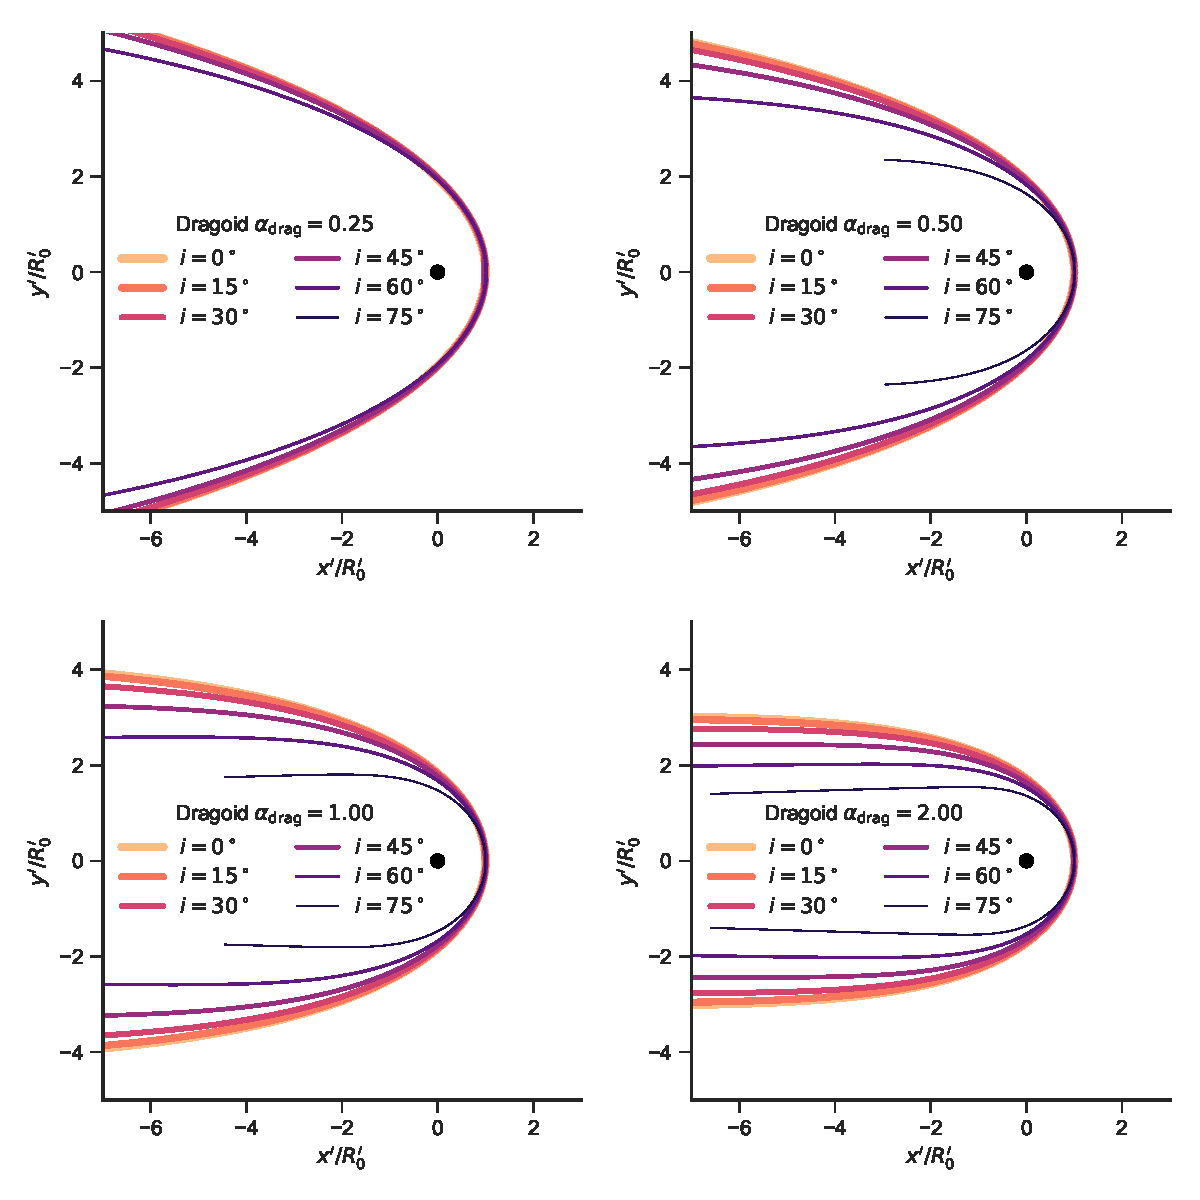
\includegraphics[width=\linewidth]{figs/test_xyprime_dragoid}
  \caption{Apparent bow shapes in the plane of the sky for
    parallel-stream dragoids as a function of inclination angle.  Drag
    coefficient, \(\alpha\drag\) increases from top-left to bottom-right.
    Inclination \(\abs{i}\) is shown in \ang{15} increments, indicated
    by line color and thickness (see key).}
  \label{fig:dragoid-xy-prime}
\end{figure}
\begin{figure}
  \centering
  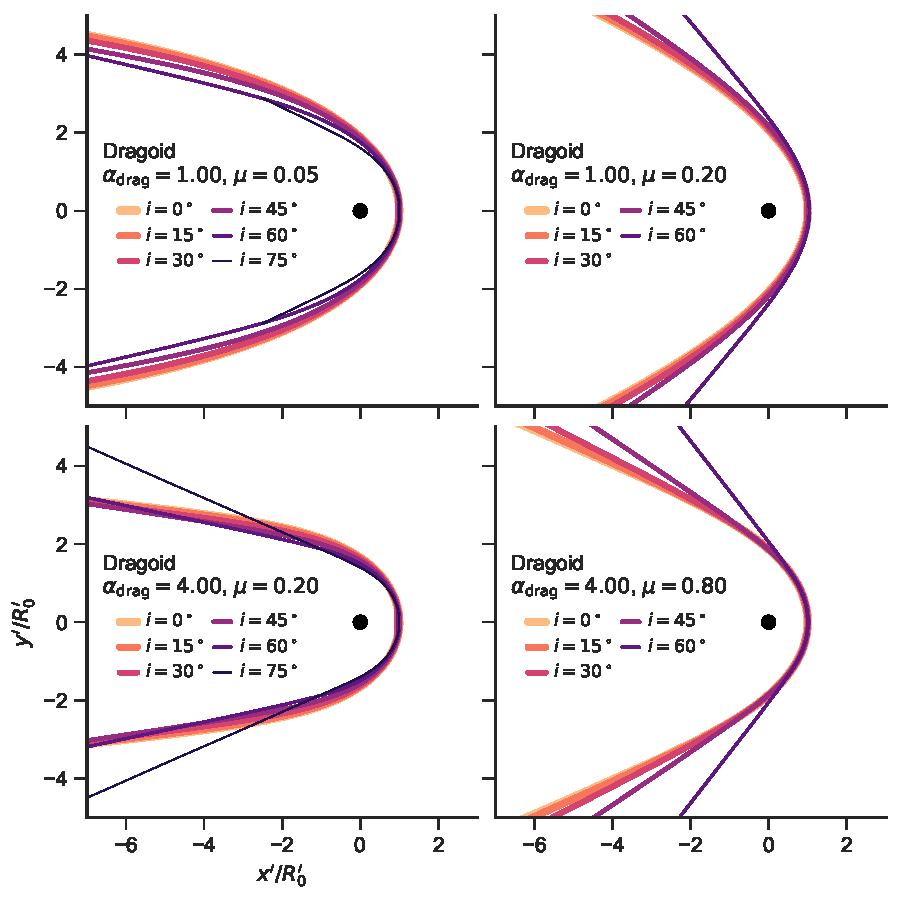
\includegraphics[width=\linewidth]{figs/test_xyprime_div_dragoid}
  \caption{As Fig.~\ref{fig:dragoid-xy-prime} but for divergent stream
    dragoids.  Drag coefficient increases from top to bottom, while
    degree of divergence increases from left to right. }
  \label{fig:dragoid-div-xy-prime}
\end{figure}


\begin{figure}
  \centering
  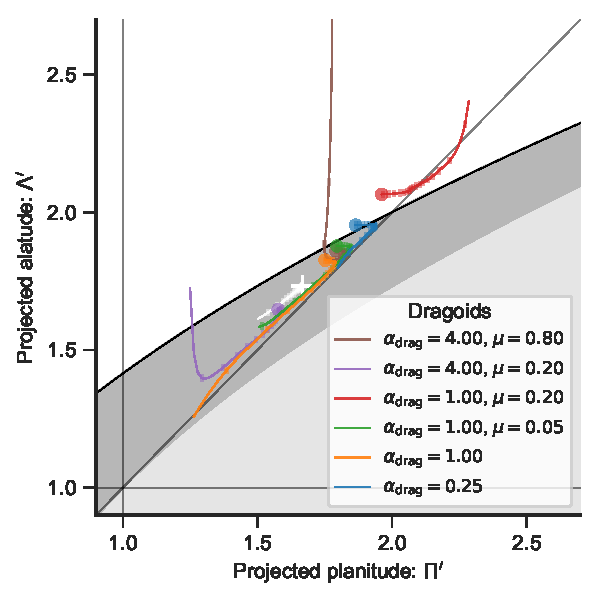
\includegraphics[width=\linewidth]{figs/dragoid-R90-vs-Rc}
  \caption{Apparent projected shapes of dragoids in the
    \(\Pi'\)--\(\Lambda'\) plane. Colored symbols indicate the
    \(\abs{i} = 0\) position for selected models (see key).  Thin
    lines show the inclination-dependent tracks of each model, with
    tick marks along each track for 20 equal-spaced values of
    \(\abs{\sin i}\). Gray shaded regions are as in
    Fig.~\ref{Q-fig:quadric-projection-continued}a of \PaperI{}.  The
    wilkinoid track is shown in white. }
  \label{fig:dragoid-Rc-R90}
\end{figure}

%%% Local Variables:
%%% mode: latex
%%% TeX-master: "dusty-bow-wave"
%%% End:

% \section{Perturbed bows}
\label{sec:perturbed-bows}

\begin{figure*}
  \centering
  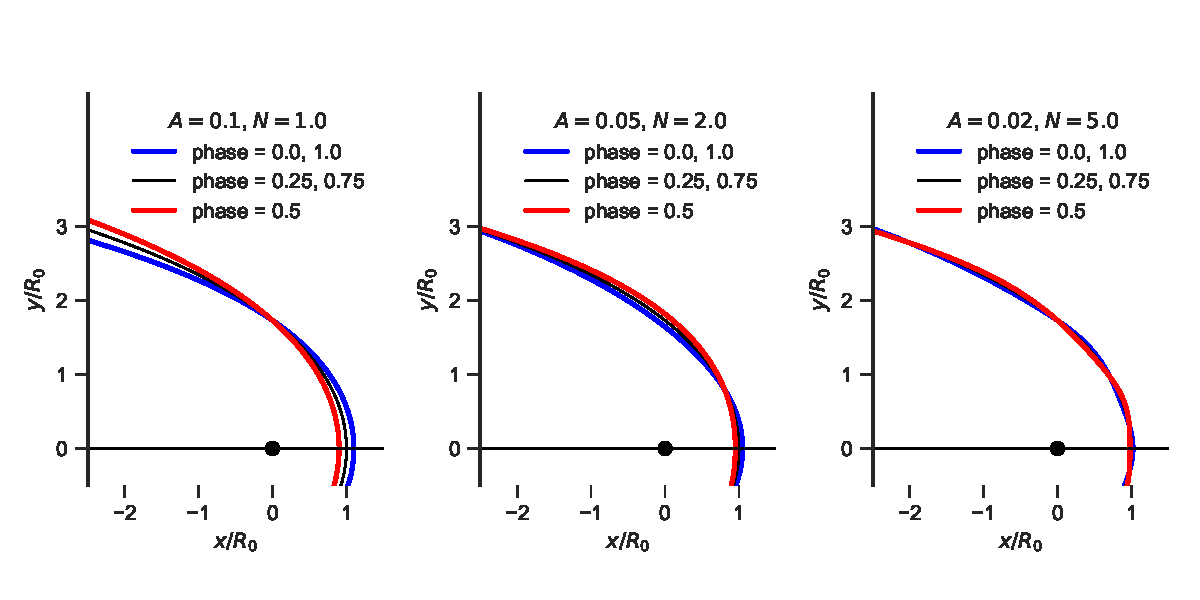
\includegraphics[width=\linewidth]{figs/compare_xyprime_wave-wilkinoid}
  \caption{Small-amplitude standing wave perturbations to bow shapes.}
  \label{fig:perturb-shapes}
\end{figure*}

\begin{figure*}
  \centering
  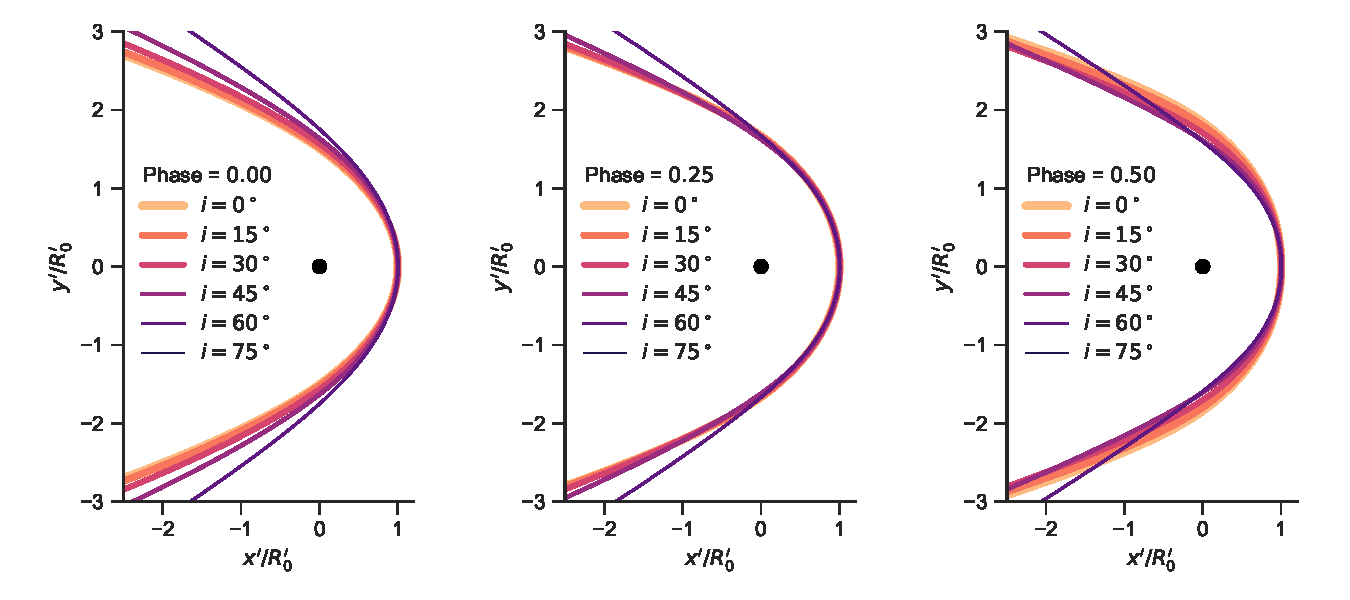
\includegraphics[width=\linewidth]
  {figs/wave_xyprime-A005-N20-ancantoid-xi080-beta000500}
  \caption{Plane-of-sky projections of perturbed bow shapes}
  \label{fig:perturb-xy-prime}
\end{figure*}

The bow shock models that we have considered so far have been
steady-state: although material is moving throughout the bow, the
pattern of its structure does not vary with time.  In this section, we
consider small, time-varying perturbations to such a steady-state
structure.  These may be due to periodic variations in the
momentum-loss rate of one of the winds, or due to dynamical
instabilities in the shocked shell.

For simplicity, we consider standing waves with an amplitude that
multiplies the bow shock radius \(R\) and a pattern that is periodic
in the axial angle \(\theta\): \(R(\theta) \to (1 + \Delta) R(\theta)\), where
\begin{equation}
  \label{eq:standing-wave}
  \Delta = A \cos(N \theta) \cos(2\pi \varphi)
\end{equation}

\begin{figure}
  \centering
  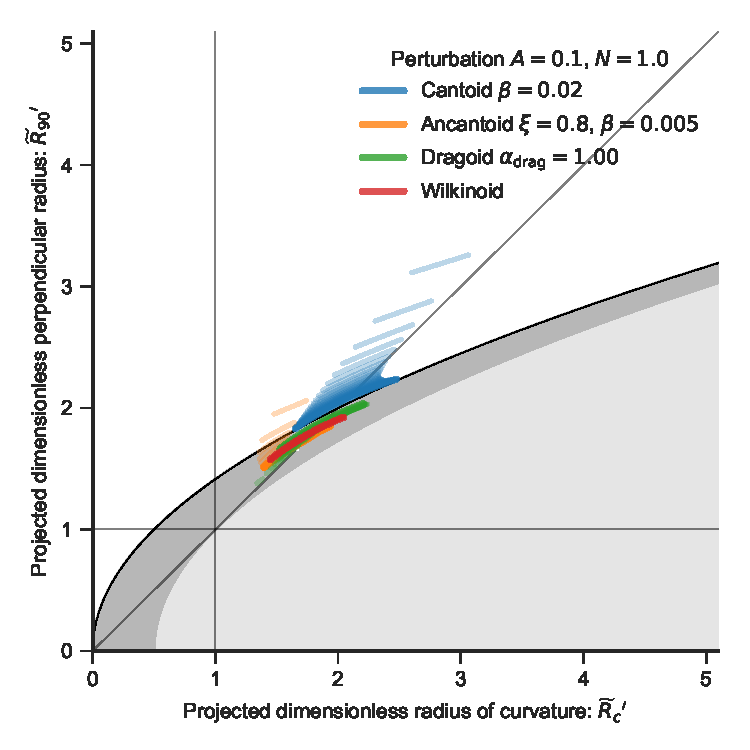
\includegraphics[width=\linewidth]
  {figs/wave-R90-vs-Rc-A010-N10}
  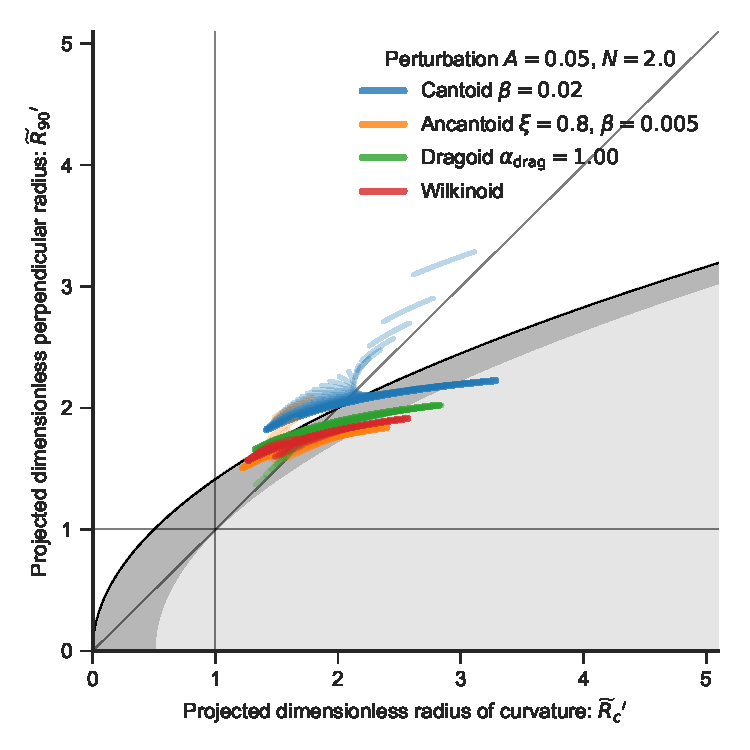
\includegraphics[width=\linewidth]
  {figs/wave-R90-vs-Rc-A005-N20}
  \caption{Diagnostic diagram for perturbed shapes}
  \label{fig:perturb-Rc-R90}
\end{figure}


%%% Local Variables:
%%% mode: latex
%%% TeX-master: "quadrics-bowshock"
%%% End:

\section{Conclusions}
\label{sec:conc}

%\newcommand\thC{\(\theta^1\)\,Ori~C}
\defcitealias{Canto:1996}{CRW}

We developed a method to estimate the shape of a generic bow shock product of the
interaction of two winds and was applied to the proplyds in the core of the ONC.
We started measuring the projected characteristic radii $(R'_0,R'_c)$ for each proplyd in our
sample and compare them with the ``conic equivalent'' of a two winds interaction model based 
on \CRW{} work to estimate the intrinsic bow shock shape and get the ionizing flux for ionization balance 
and the stagnation pressure for our sample of proplyds.
Most results are consistent with a proplyd's photoevaporated flow with an anisotropic density
distribution, with different anisotropy degrees. We ound that LV4 has the least anisotropic flow,
while LV2 has the most anisotropic flow. And for the 177-341, 169-348 and 180-331 we found out that 
the stellar wind is not enough to keep their bow socks stationary.

%%% Local Variables:
%%% mode: latex
%%% TeX-master: "proplyd-bowshocks"
%%% End:

\bibliographystyle{mnras}
%% All references should be put in the BibTeX file bowshocks-biblio.bib
\bibliography{bowshocks-biblio}
\appendix
\section{Paraboloids and their plane-of-sky projection}
\label{app:parabola}

Equation~\eqref{eq:par-xy} for the \(xy\) coordinates of a quadric in the \(\phi = 0\) plane cannot be used in the case of a paraboloid (\(\Q = 0\)).  Instead, a convenient parametrization is
\begin{gather}
  \label{eq:parabola-xy}
  \begin{aligned}
    x &= R_0 \left(1  - \tfrac{1}{2} \Pi\, t^2\right) \\
    y &= R_0\, \Pi\, t \ ,
  \end{aligned}
\end{gather}
where we have ``baked in'' knowledge of the planitude,
\(\Pi = R_{\C}/R_0\) (see \S~\ref{sec:plan-alat-bow}). The projected
plane-of-sky coordinates of the tangent line follow from
equation~\eqref{eq:Trans} as
\begin{gather}
  \label{eq:parabola-xy-prime-phi}
  \begin{aligned}
    x_{\T}' / R_0 &= \left(1 - \tfrac{1}{2} \Pi\, t^2\right) \cos i
      + \Pi\, t \sin\phi_{\T} \sin i\\
    y_{\T}' / R_0 &= \Pi\, t \cos\phi_{\T}\ ,
  \end{aligned}
\end{gather}
The azimuth of the tangent line is found from
equations~(\ref{eq:alpha}, \ref{eq:tanphi}) as
\(\sin\phi_{\T} = -t^{-1} \tan i \), so that
\begin{gather}
  \label{eq:parabola-xy-prime-final}
  \begin{aligned}
    x_{\T}' / R_0 &= \cos i \left[ 1 + \tfrac{1}{2} \Pi \tan^2 i -
      \tfrac{1}{2} \Pi \left( t^2 - \tan^2 i \right) \right]\\
    y_{\T}' / R_0 &= \Pi \left( t^2 - \tan^2 i \right)^{1/2} \ .
  \end{aligned}
\end{gather}
The projected star--apex distance, \(R_0'\), is the value of
\(x_{\T}'\) when \(y_{\T}' = 0\), yielding
\begin{equation}
  \label{eq:parabola-R0-prime}
  R_0' / R_0 = \cos i \left( 1 + \tfrac{1}{2} \Pi \tan^2 i  \right) \ . 
\end{equation}
Note that this same result can be obtained from a Taylor expansion of
equation~\eqref{eq:fQi-factor} substituted into~\eqref{eq:R0-prime} in
the limit \(\Q \to 0\).

Equation~\eqref{eq:parabola-xy-prime-final} can be rewritten in the
form
\begin{gather}
  \label{eq:parabola-xy-all-primes}
  \begin{aligned}
    x_{\T}' &= R_0' \left(1  - \tfrac{1}{2} \Pi' t'^2\right) \\
    y_{\T}' &= R_0' \Pi' t' \ ,
  \end{aligned}
\end{gather}
where
\begin{align}
  \label{eq:parabola-Pi-prime}
  \Pi' &= \frac{2 \Pi} {2 \cos^2 i + \Pi \sin^2 i} \\
  \label{eq:parabola-t-prime}
  t' &= \cos i \left(t^2 - \tan^2 i\right)^{1/2} \ ,
\end{align}
which demonstrates that the projected shape is also a parabola. It is
apparent from \eqref{eq:parabola-Pi-prime} that the projected
planitude obeys
\begin{equation*}
\lim_{i \to 90^\circ} \Pi' = 2 \ ,
\end{equation*}
for all values of the true planitude \(\Pi\), as is shown by the black
lines in Figure~\ref{fig:quadric-projection}a. The projected alatude can
be found as
\begin{equation}
  \label{eq:parabola-Lambda-prime}
  \Lambda' = \left( 2 \Pi' \right)^{1/2} \ .
\end{equation}
For the special case of the confocal paraboloid,
\(\Pi = \Lambda = 2\), we have \(\Pi' = \Pi\) and
\(\Lambda' = \Lambda\) by equations~\eqref{eq:parabola-Pi-prime}
and~\eqref{eq:parabola-Lambda-prime} for all inclinations, so its
shape is unaffected by projection.
%%% Local Variables:
%%% mode: latex
%%% TeX-master: "quadrics-bowshock"
%%% End:


\section{Bow shocks from anisotropic wind--wind interactions}
\label{app:ancantoid}
\begin{figure}
  \centering
  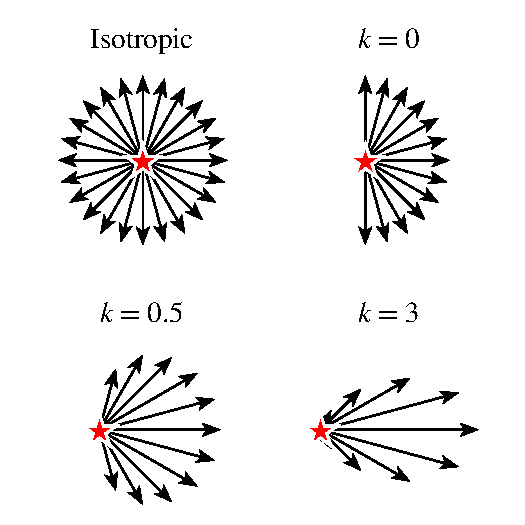
\includegraphics[width=\linewidth]{figs/anisotropic-arrows}
  \caption[]{Schematic diagram of wind flow patterns in isotropic and
    non-isotropic cases for different values of the anisotropy index,
    \(k\).  Arrow length represents the wind momentum loss rate per
    solid angle.}
  \label{fig:anisotropic-arrows}
\end{figure}


We wish to generalize the results of \citet[\CRW{}]{Canto:1996} to the
case where the inner wind is no longer isotropic, but instead has a
density that falls off with angle, \(\theta\), away from the symmetry axis.
Specifically, at some fiducial radius, \(r_0\), from the origin, the
wind mass density is given by
\begin{equation}
  \label{eq:ancantoid-density}
  \rho(r_0, \theta) =
  \begin{cases}
    \rho_0 \cos^k \theta & \text{for \(\theta \le 90^\circ\)} \\
    0 & \text{for \(\theta > 90^\circ\)}
  \end{cases}
  \ ,
\end{equation}
where \(\rho_0\) is the density on the symmetry axis and \(k \ge 0\) is an
\textit{anisotropy index}.  The wind velocity is still assumed to be
constant and the wind streamlines to be radial, so the radial
variation of density at each angle is
\(\rho(r, \theta) = \rho(r_0, \theta)\, (r/r_0)^{-2}\) and the wind mass loss rate and
momentum loss rate per solid angle both have the same \(\cos^k\theta\)
dependence as the density.  Examples are shown in
Figure~\ref{fig:anisotropic-arrows} for a variety of different values
of \(k\).  As \(k\) increases, the wind becomes increasingly jet-like.

Our primary motivation for considering such an anisotropic wind is the
case of the Orion Nebula proplyds and their interaction with the
stellar wind of the massive star \thC{}
\citep{Garcia-Arredondo:2001a}.  The inner ``wind'' in this case is
the transonic photoevaporation flow away from a roughly hemispherical
ionization front, where photoionization equilibrium, together with
monodirectional illumination of the front, implies that the ionized
hydrogen density, \(n\), satisfies \(n^2 \propto \cos \theta\), which is
equivalent to \(k = 0.5\) in equation~\eqref{eq:ancantoid-density}.
Since the primary source of ionizing photons is the same star that is
the source of the outer wind, it is natural that the inner wind's axis
should be aligned with the star--star axis in this case.  For other
potential causes of wind anisotropy (for instance, bipolar flow from
an accretion disk), there is no particular reason for the axes to be
aligned, so cylindrical symmetry would be broken.  Nevertheless, we
calculate results for general \(k\) with aligned axes, so as to
provide a richer variety of cylindrically symmetric bow shock shapes
than are seen in the cantoids.

The general solution for the bow shock shape, \(R(\theta)\), in the \CRW{}
formalism is
\begin{equation}
  R(\theta) = \frac {\dot{J}_{\w} + \dot{J}_{\w{}1}}
  {\left(\dot{\Pi}_{\w{}r}+\dot{\Pi}_{\w{}r1}\right)\cos\theta
    - \left(\dot{\Pi}_{\w{}z}+\dot{\Pi}_{\w{}z1}\right)\sin\theta}
  \label{eq:Rmom}
\end{equation}
where \(\dot{\Pi}_{\w{}r}\), \(\dot{\Pi}_{\w{}z}\), \(\dot{J}_{\w}\) are
the accumulated linear radial momentum, linear axial momentum, and
angular momentum, respectively, due to the inner wind emitted between
the axis and \(\theta\). The equivalent quantities for the outer wind have
subscripts appended with ``1''.  The inner wind momenta for our
anisotropic case (replacing \CRW{}'s eqs.~[9, 10]) are:
\begin{gather}
  \label{eq:ancantoid-momenta}
  \begin{aligned}
    \dot{\Pi}_{\w{}z} &= \frac{k + 1}{2(k+2)}\, \dot{M}_{\w}^0 V_{\w}
    \left(1-\cos^{k+2}\theta\right) \\
    \dot{\Pi}_{\w{}r} &= (k + 1)\, \dot{M}^0_{\w} V_{\w}\, I_k (\theta) 
  \end{aligned}
\end{gather}
where
\begin{equation}
  \label{eq:ancantoid-mass-loss}
  \dot{M}^0_{\w} = \frac{2 \pi} {k + 1} r_0^2 \rho_0 V_{\w}
\end{equation}
is the total mass-loss rate of the inner wind. The integral
\begin{equation}
  \label{eq:ancantoid-I-integral}
  I_k(\theta) = \int^\theta_0 \cos^k \theta \sin^2\theta \,d\theta 
\end{equation}
has an analytic solution in terms of the hypergeometric function,
\({}_2 F_1(-\tfrac12; \tfrac{1+k}2; \tfrac{3+k}2; \cos^2 \theta)\), but is
more straightforwardly calculated by numerical quadrature.  The
angular momentum of the inner wind about the origin is
\(\dot{J}_{\w} = 0\) because it is purely radial.  The outer wind
momenta are unchanged from the \CRW{} case, but are given here for
completeness:
\begin{gather}
  \label{eq:ancantoid-momenta-outer}
  \begin{aligned}
    \dot{\Pi}_{\w{}z1} & =
    -\frac{\dot{M}^0_{\w{}1}V_{\w{}1}}{4}\sin^2\theta_1\\
    \dot{\Pi}_{\w{}r1} & =
    \frac{\dot{M}^0_{\w{}1}V_{\w{}1}}{4}\left(\theta_1-\sin\theta_1\cos\theta_1\right)\\
    \dot{J}_{\w{}1} & =
    \frac{\dot{M}^0_{\w{}1}V_{\w{}1}}{4}\left(\theta_1-\sin\theta_1\cos\theta_1\right)D \ .
  \end{aligned} 
\end{gather}

We define \(\beta\) in this case as the momentum ratio \emph{on the symmetry axis}, which means that 
\begin{equation}
  \label{eq:ancantoid-momentum-ratio}
  \dot{M}^0_{\w{}1}V_{\w{}1} = 2 (k + 1)\, \beta\, \dot{M}^0_{\w} V_{\w} \ . 
\end{equation}
Substituting
equations~(\ref{eq:ancantoid-momenta}--\ref{eq:ancantoid-momentum-ratio})
into equation~\eqref{eq:Rmom} and making use of the geometric relation
between the interior angles of the triangle shown in
Figure~\ref{fig:crw-schema}:
\begin{equation}
  \label{eq:crw-angles}
  R \sin(\theta + \theta_1) = D \sin \theta_1 \ , 
\end{equation}
yields
\begin{equation}
  \label{eq:ancantoid-theta-theta1-implicit}
  \theta_1 \cot \theta_1 = 1 +
  2 \beta \left(
    I_k(\theta) \cot \theta
    - \frac{1 - \cos^{k+2} \theta} {k + 2} \right)   \ , 
\end{equation}
which is the generalization of \CRW{}'s equation~(24) to the
anisotropic case.  Equation~\eqref{eq:ancantoid-theta-theta1-implicit}
is solved numerically to give \(\theta_1(\theta)\), which is then combined with
equations~(\ref{eq:crw-angles}) and (\ref{eq:stagnation-radius}) to
give the dimensionless bow shape, \(R(\theta; \beta, k)/R_0\), where we now
explicitly indicate the dependence of the solution on two parameters:
axial momentum ratio, \(\beta\), and anisotropy index, \(k\).  We refer to
the resultant bow shapes as \textit{ancantoids}.



%The most notable scenarios, since they have astrophysical relevance are the following:
%$k=1/2$ ak.a. the ``proplyd case'', following \citep{HA:1998}, and $k=0$, ak.a, the ``isotropic case'', following \CRW{}. The comparison between both solutions
%is shown in figure (\ref{fig:r-beta}), along with an extreme anisotropy case. 

%%% Local Variables:
%%% mode: latex
%%% TeX-master: "quadrics-bowshock"
%%% End:

\section{Analytic derivation of thin-shell bow shape parameters}
\label{sec:thin-shell-shapes}

In this appendix, we provide analytic calculations of the planitude,
alatude, and asymptotic opening angle for the wilkinoid, cantoids, and
ancantoids.  We first consider the most general case of the
ancantoids, and then show how results for cantoids and the wilkinoid
follow as special cases.

\subsection{Planitude of ancantoids}
\label{sec:ancantoid-planitude}

From equations~\eqref{eq:radius-curvature} and~\eqref{eq:planitude},
the planitude depends on the apex second derivative,
\(R_{\theta\theta,0}\), as
\begin{equation}
  \label{eq:planitude-from-2nd-derivative}
  \Pi = \left(  1 - R_{\theta\theta,0} / R_0\right)^{-1} \ .
\end{equation}
From equation~\eqref{eq:taylor-R-theta}, the second derivative can be
found from the coefficient of \(\theta^2\) in the Taylor expansion
of \(R(\theta)\).  Since we do not have \(R(\theta)\) in explicit analytic form,
we proceed via a Taylor expansion of the implicit
equations~\eqref{eq:crw-angles}
and~\eqref{eq:ancantoid-theta-theta1-implicit}, retaining terms up to
\(\theta^4\) to obtain from
equation~\eqref{eq:ancantoid-theta-theta1-implicit}:
\begin{equation}
  \label{eq:taylor-expansion-implicit}
  \theta_1^2 = \beta \theta^2 \left( 1 + C_{k\beta} \theta^2\right) + \mathcal{O}(\theta^6)\ , 
\end{equation}
with the coefficient \(C_{k\beta}\) given by
\begin{equation}
  \label{eq:C-k-beta}
  C_{k\beta} = \frac{1}{15} - \frac{3k}{20} - \frac{\beta}{15}  \ .
\end{equation}
Note that it is necessary to include the \(\theta^4\) term in the expansion
of \(\theta_1^2\) so that \(\theta_1/\theta\) is accurate to order
\(\theta^2\).  Then, from equation~\eqref{eq:crw-angles} we find
\begin{align}
  \label{eq:taylor-R-over-D}
  \frac{R}{D} & = \frac{\sin \theta_1} {\sin (\theta + \theta_1)} \nonumber \\
              & = \frac{\beta^{1/2}}{1+\beta^{1/2}}
                \left\lbrace 1 + \theta^2
                \left[ \frac{C_{k\beta}} {2 \left(1+\beta^{1/2}\right)}
                + \frac{1}{6} \left(1+2\beta^{1/2} \right)
                \right]
                \right\rbrace + \mathcal{O}(\theta^4) \ ,
\end{align}
where in the second line we have carried out a Taylor expansion of the
two \(\sin\) terms and substituted
\eqref{eq:taylor-expansion-implicit}.  Comparing coefficients of unity
and \(\theta^2\) between equations~\eqref{eq:taylor-R-theta} and
\eqref{eq:taylor-R-over-D} we find
\begin{align}
  \label{eq:again-R0-over-D}
  \frac{R_0} {D} &= \frac{\beta^{1/2}}{1+\beta^{1/2}} \\
  \label{eq:final-second-derivative}
  \frac{R_{\theta\theta,0}} {R_0} &= \frac{C_{k\beta}}{1+\beta^{1/2}}+\frac{1}{3}\left(1+2\beta^{1/2}\right) \ ,
\end{align}
so that the final result for the planitude, from~\eqref{eq:planitude-from-2nd-derivative}, is
\begin{equation}
  \label{eq:final-planitude}
  \text{ancantoid} \quad
  \Pi = \left[ {1 - \frac{C_{k\beta}}{1+\beta^{1/2}} - \frac{1}{3}\left(1+2\beta^{1/2}\right)}
  \right]^{-1} \ .
\end{equation}

\subsection{Alatude of ancantoids}
\label{sec:ancantoid-alatude}

To find the alatude, \(\Lambda = R_{90} / R_0\), we use
equation~\eqref{eq:crw-angles} at \(\theta = \ang{90}\) to write
\begin{equation}
  \label{eq:Lambda-from-theta-1-90}
  \Lambda = \frac{D} {R_0} \tan \theta_{1,90} \ , 
\end{equation}
where \(\theta_{1,90} = \theta_1(\theta = \ang{90})\), which, following
equation~\eqref{eq:ancantoid-theta-theta1-implicit}, must satisfy
\begin{equation}
  \label{eq:theta-1-90-implicit}
  \theta_{1,90} \cot \theta_{1,90}  = 1 - \frac{2 \beta}{k + 2} \ . 
\end{equation}
Combining \eqref{eq:Lambda-from-theta-1-90} and
\eqref{eq:theta-1-90-implicit} with \eqref{eq:again-R0-over-D} yields
\begin{equation}
  \label{eq:Lambda-beta-xi-theta-1-90}
  \Lambda = \frac{ \left(1 + \beta^{1/2}\right) \,\theta_{1,90}} {\beta^{1/2} \left(1 - \xi_k \beta\right)} \ ,
\end{equation}
where
\begin{equation}
  \label{eq:xi-k}
  \xi_k = \frac{2} {k +2} \ .
\end{equation}
We now take the Taylor expansion of equation~\eqref{eq:theta-1-90-implicit} to find
\begin{equation}
  \label{eq:theta-1-90-Taylor}
  \theta_{1,90}^2 + \tfrac{1}{15}  \theta_{1,90}^4 + \mathcal{O}(\theta_{1,90}^6)
  = 3 \xi_k \beta \ , 
\end{equation}
which, if \(\theta_{1,90}\) is small, has the approximate solution
\begin{equation}
  \label{eq:theta-1-90-approx}
  \theta_{1,90} \approx \left( \frac{3 \xi_k \beta} {1 + \tfrac15 \xi_k \beta} \right)^{1/2} \ .
\end{equation}
Substituting back into equation~\eqref{eq:Lambda-from-theta-1-90}
yields an approximate value for the alatude of
\begin{equation}
  \label{eq:Lambda-approx}
  \text{ancantoid} \quad
  \Lambda \approx \frac {(3 \xi_k)^{1/2} \left( 1 + \beta^{1/2} \right)}
  { \left( 1 + \tfrac15 \xi_k \beta \right)^{1/2} \left( 1 - \xi_k \beta \right)} \ .
\end{equation}
This approximation is surprisingly accurate, with a relative error of
order \(1\%\) even for \(\beta\) as large as \(0.5\) with \(k = 0\).  

\subsection{Planitude and alatude of cantoids and wilkinoid}
\label{sec:cantoid-wilkinoid-shapes}

Since \(\Pi\) and \(\Lambda\) depend on only that portion of the inner wind
emitted in the forward hemisphere, \(\theta \le \ang{90}\), the results for the
cantoids can be found by taking \(k = 0\), in which case
equations~(\ref{eq:C-k-beta}, \ref{eq:final-planitude}, \ref{eq:xi-k},
\ref{eq:Lambda-approx}) yield
\begin{gather}
  \label{eq:cantoid-Pi-Lambda}
  \text{cantoid} \quad
  \begin{cases}
    \quad \Pi &= \dfrac {5} {3 \left( 1 - \beta^{1/2} \right)}\\[12pt]
    \quad \Lambda &= \dfrac { \sqrt 3} {\left( 1 + \tfrac15 \beta \right)^{1/2} \left( 1 - \beta^{1/2} \right)} \ .
  \end{cases}
\end{gather}
The wilkinoid shape is equal to the \(\beta \to 0\) limit of the cantoid, so
its planitude and alatude are given by:
\begin{gather}
  \label{eq:wilkinoid-Pi-Lambda}
  \text{wilkinoid} \quad
  \begin{cases}
    \quad \Pi &= \dfrac {5} {3}\\[10pt]
    \quad \Lambda &= \sqrt 3 \ .
  \end{cases}
\end{gather}
The wilkinoid results can also be obtained directly from
equation~\eqref{eq:wilkinoid-R-theta}, and in the case of \(\Lambda\) this
has already been noted by several authors \citep{Cox:2012a,
  Meyer:2016a}.

\subsection{Asymptotic opening angle}
\label{sec:asympt-open-angle}

The asymptotic opening angle
of the far wings, \(\theta_\infty\), can be found from
equation~\eqref{eq:ancantoid-theta-theta1-implicit} for the
ancantoids, together with the condition that
\(\theta_\infty + \theta_{1\infty} = \pi\).  These yield the implicit equation
\begin{equation}
  \label{eq:ancantoid-theta-inf}
  \theta_\infty - \left( \frac {k + 2 (1 - \beta)} {k + 2} \right) \tan \theta_\infty
  = \pi + 2 \beta I_k(\pi/2) \ ,
\end{equation}
where
\begin{equation}
  I_k(\pi/2) = \frac{\sqrt \pi}{4} \,
      \frac{  \GammaFunc\left( \frac{k+1}{2} \right)} {\GammaFunc\left(\frac{k+4}{2}\right)}
\end{equation}
and \(\GammaFunc\) is the usual Gamma function.  This can be compared with the equivalent result obtained by \CRW{} for the cantoids:
\begin{equation}
  \label{eq:cantoid-theta-inf}
  \theta_\infty - \tan \theta_\infty = \frac{\pi}{1 - \beta} \ .
\end{equation}
Note that, unlike in the cases of \(\Pi\) and \(\Lambda\),
equation~\eqref{eq:ancantoid-theta-inf} does \emph{not} reduce to
equation~\eqref{eq:cantoid-theta-inf} in the limit \(k \to 0\).  This is
because, for \(\theta > \ang{90}\), the \(k = 0\) ancantoid differs from the
cantoid since the former has no wind in the backward hemisphere (see
Figure~\ref{fig:anisotropic-arrows}).  Therefore there is less inner
support for the far wings of the bow, and so \(\theta_\infty\) is smaller than
in the cantoid case.  The wilkinoid result again follows from
\(\beta \to 0\), implying that \(\theta_\infty = \pi\), or, in other words, that the far
wings are asymptotically parallel to the symmetry axis, as is the case
for the paraboloid (App.~\ref{app:parabola}).  In the case of the
wilkinoid, however, the behavior is cubic in the wings,
\(z \sim r^3\), as opposed to quadratic as in the paraboloid.
%%% Local Variables:
%%% mode: latex
%%% TeX-master: "quadrics-bowshock"
%%% End:

% \section{Equations of motion for grains with radiation and gas drag}
\label{sec:equat-moti-grains}

\begin{figure}
  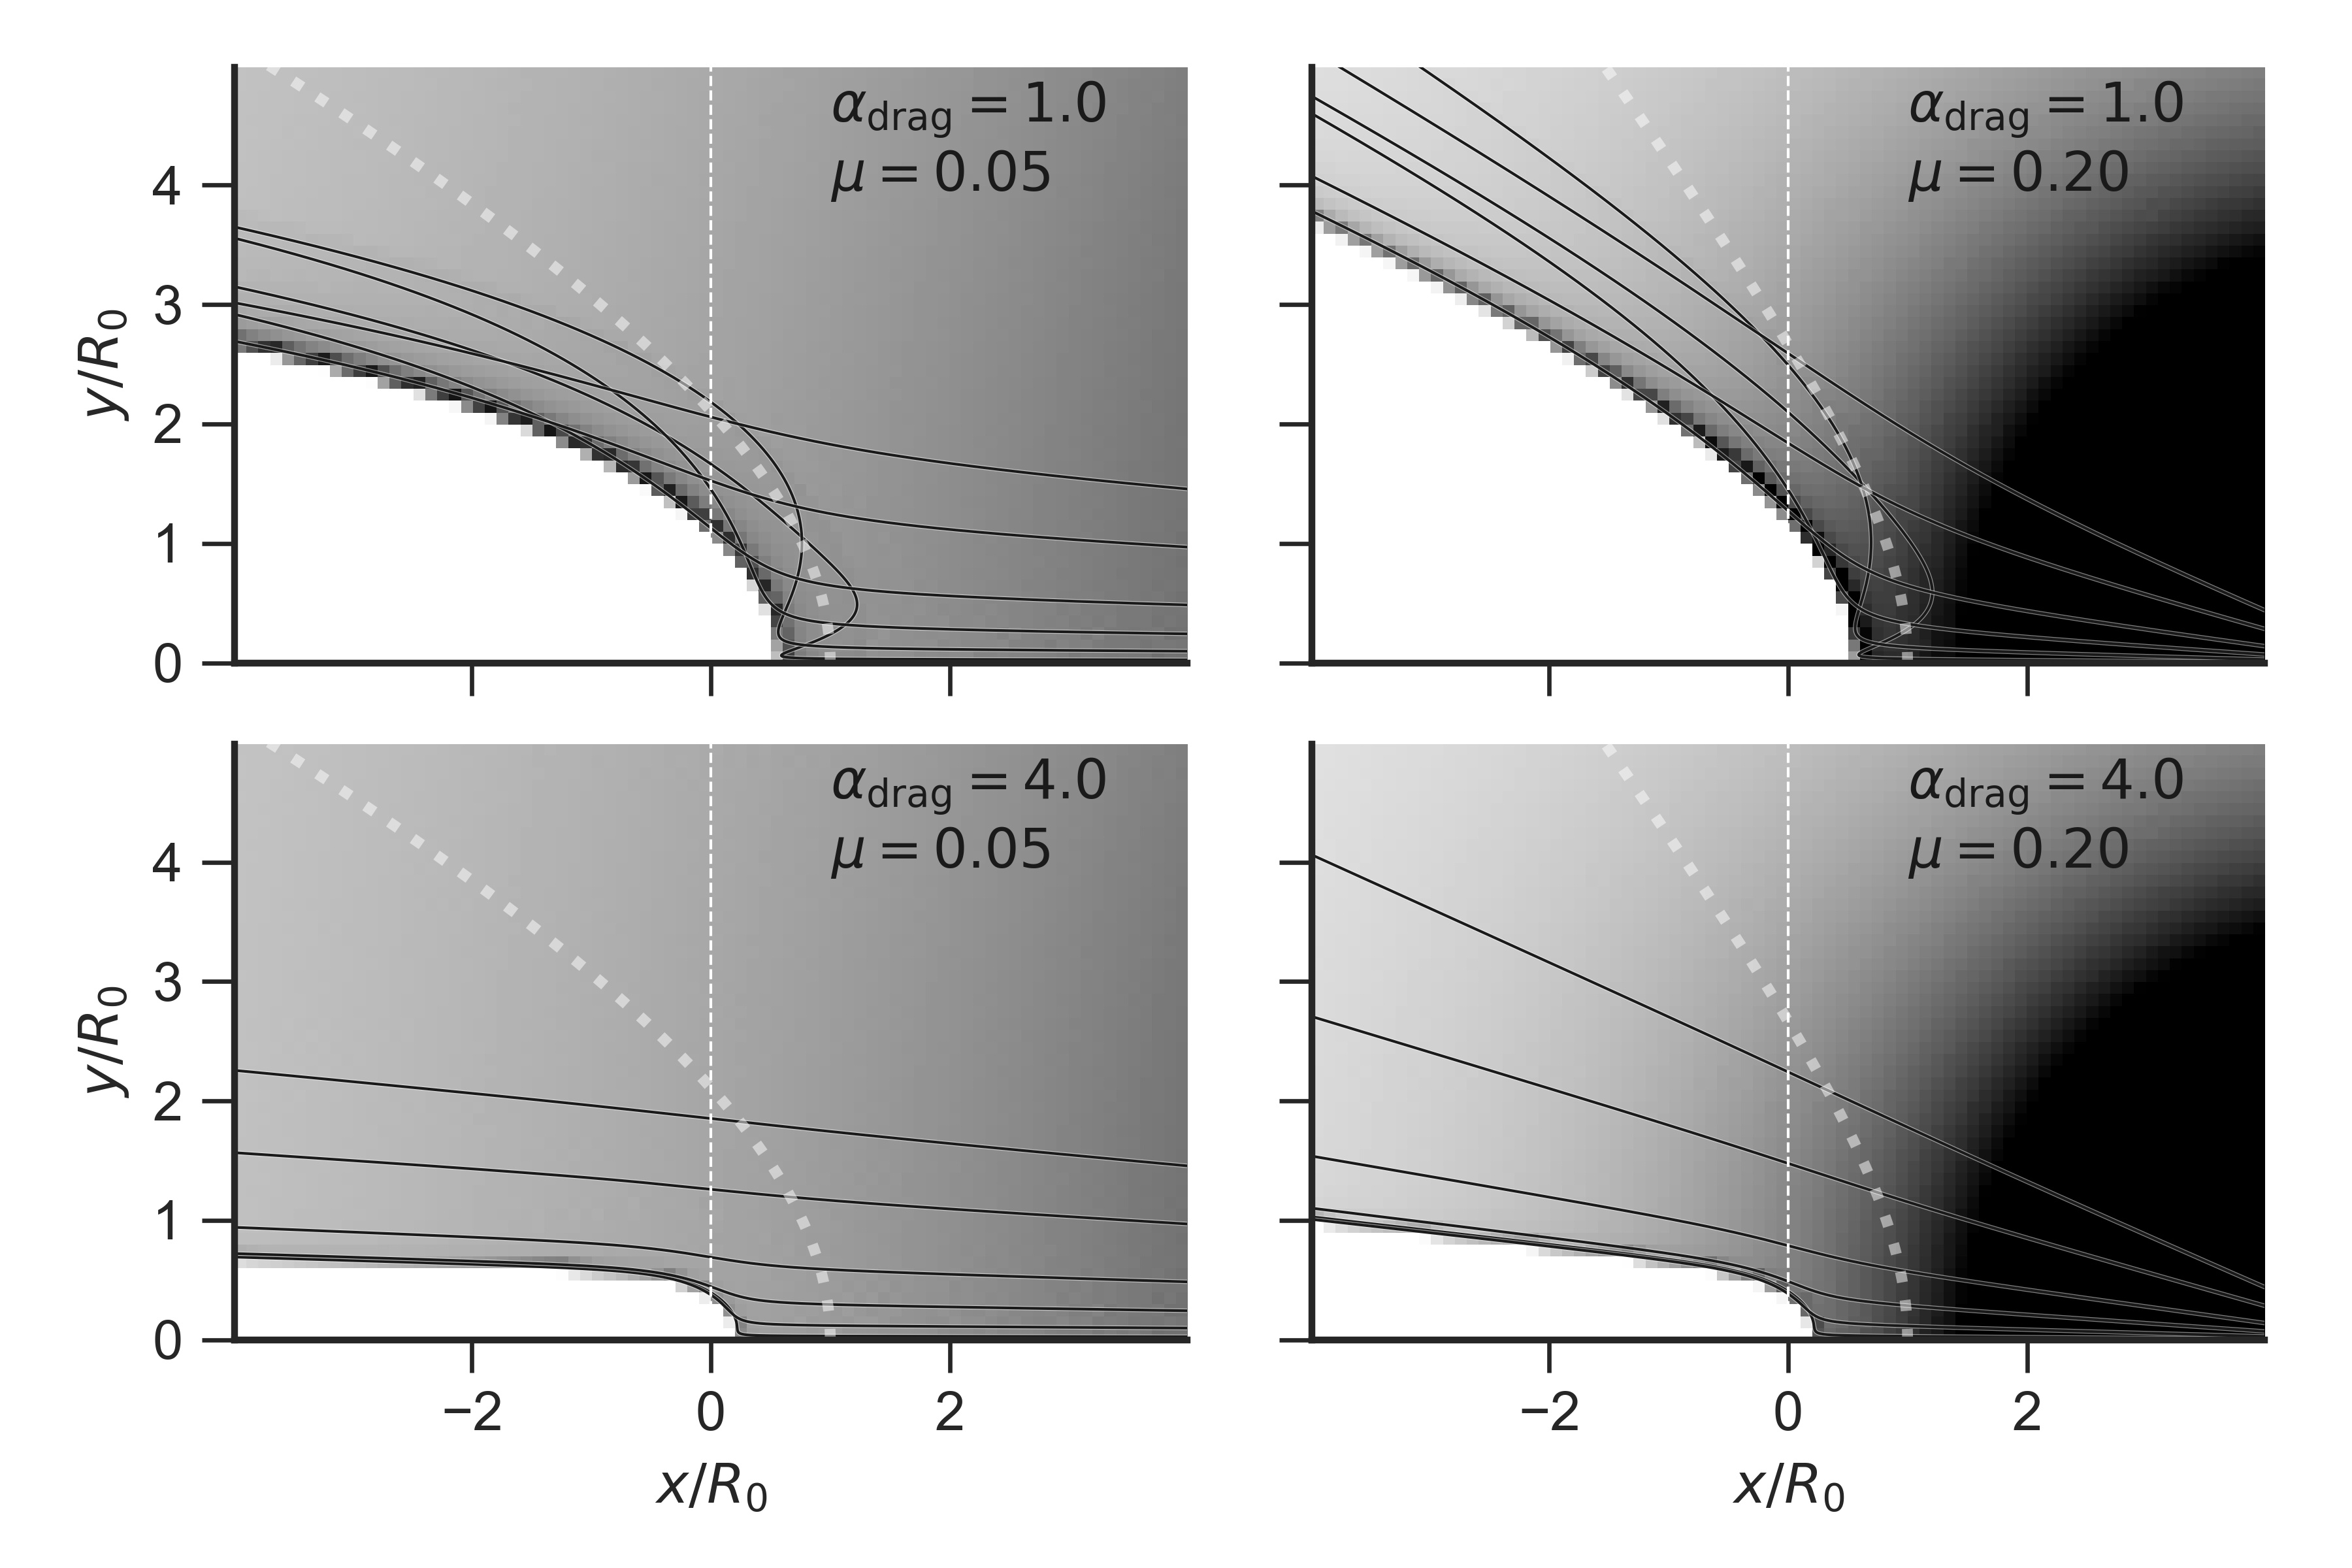
\includegraphics[width=\linewidth]{figs/dust-couple-div-stream}
  \caption{Divergent dragoids}
  \label{fig:divergent-dragoids}
\end{figure}

To find the dust grain trajectories \(R\grain(\theta)\) in the presence of
radiation and drag forces (\S~\ref{sec:bow-wave-drag}), we numerically
integrate the equations of motion. We define dimensionless cylindrical
polar coordinates,
\begin{equation}
  \label{eq:dust-XY}
  (X, Y) = \left(\frac{R\grain(\theta) \cos\theta } {R_0}, \ 
    \frac{R\grain(\theta) \sin\theta } {R_0}\right)
  \ ,
\end{equation}
and dust grain velocities,
\begin{equation}
  \label{eq:dust-UV}
  (U, V) = \left( \frac{\bm{v}\grain \cdot \uvec{x}} {v_\infty}, \ 
  \frac{\bm{v}\grain \cdot \uvec{y}} {v_\infty}\right) \ ,
\end{equation}
where \(\uvec{x}\) and \(\uvec{y}\) are unit vectors along the \(X\)
and \(Y\) axes (parallel and perpendicular, respectively, to the
symmetry axis).  The grain equation of motion then follows from
equations~(\ref{eq:dust-rad-force}, \ref{eq:dust-r0},
\ref{eq:dust-fdrag}--\ref{eq:dust-alpha}) as the following set of
coupled differential equations:
\begin{gather}
  \label{eq:dust-motion}
  \begin{aligned}
    \frac{d X}{d t} &= U \quad\quad
    \frac{d Y}{d t} = V \\
    \frac{d U}{d t} &= \frac12 \left[  
      X \left(X^2 + Y^2\right)^{-3/2} - \alpha\drag^2 D_1 \left(U - U_1\right)
    \right] \\
    \frac{d V}{d t} &= \frac12 \left[  
      Y \left(X^2 + Y^2\right)^{-3/2} - \alpha\drag^2 D_1 \left(V - V_1\right)
    \right] \ ,
  \end{aligned}
\end{gather}
where \((U_1, V_1)\) are the components of the gas velocity (assumed
fixed), given by
\begin{equation}
  \label{eq:dust-gas-velocities}
  (U_1, V_1) = 
  \begin{cases}
    \text{parallel stream} & (-1, 0)\\
    \text{divergent stream} &
    \left( \dfrac{X - \mu^{-1}}{R_1},\ \dfrac{Y}{R_1}\right) \ ,
  \end{cases}
\end{equation}
where
\begin{equation}
  \label{eq:dust-R1}
  R_1 = \left( \bigl(X - \mu^{-1}\bigr)^2 + Y^2 \right)^{1/2}
\end{equation}
is the distance from the second source, located at
\((X, Y) = (\mu^{-1}, 0)\).  The dimensionless gas density, \(D_1\),
normalized by the value at \((X, Y) = (1, 0)\), is
\begin{equation}
  \label{eq:dust-gas-density}
  D_1 = 
  \begin{cases}
    \text{parallel stream} & 1\\
    \text{divergent stream} & \dfrac{\bigl(\mu^{-1} - 1\bigr)^2} {R_1^{2}} \ .
  \end{cases}
\end{equation}

Equations~\eqref{eq:dust-motion} are integrated using the python
wrapper \texttt{scipy.integrate.odeint} to the Fortran ODEPACK library
\citep{Hindmarsh:1983a, Jones:2001a}, with results shown in
Figure~\ref{fig:dust-wave-coupling} for parallel-stream cases and
Figure~\ref{fig:divergent-dragoids} for divergent-stream cases. 

%%% Local Variables:
%%% mode: latex
%%% TeX-master: "dusty-bow-wave"
%%% End:


% Don't change these lines
\bsp	% typesetting comment
\label{lastpage}
\end{document}

%%% Local Variables:
%%% mode: latex
%%% TeX-master: t
%%% End:

